\chapter{Sequence Analysis of Ribosomal Step Parameters}
%\bibliographystyle{nar}
\label{sequence} 

For the 2007 IMA Meeting, ``RNA in Biology, Bioengineering and
Nanotechnology'', that took place from October 29 to November 2, 2007 in
Minneapolis, Minnesota, we sorted the base-steps of rRNA
according to 16 possible sequence base-steps, that is, Purine-Purine
(RR: AA, AG, GA, GG), Pyrimidine-Pyrimidine (YY: UU, UC, CU, CC),
Pyrimidine-Purine (YR: UA, UG, CA, CG), and Purine-Pyrimidine (RY: AU,
AC, GU, GC).
In Table~\ref{tab:distribution} we show how these 16 base-steps
distribute in the complete rRNA structure (All), in the helical regions of
rRNA found by the 3DNA software (Helical), and in base-steps whose
first member is part of a Watson-Crick (WC) base-pair.

\begin{table}[htbp]
\begin{center}
{\small
%\begin{tabular}{|c|p{1cm}|c|c|c|}
\begin{tabular}{|c|c|c|c|c|}
\hline
\multicolumn{2}{|c|}{Ribosome  50S}& All & Helical & Watson-Crick \\ \hline
RR & AA & 202 & 102 & 12  \\ \hline
   & AG & 232 & 164 & 60  \\ \hline
   & GA & 250 & 177 & 64  \\ \hline
   & GG & 249 & 238 & 160 \\ \hline
YY & UU & 75  & 54  & 20  \\ \hline
   & UC & 147 & 107 & 66  \\ \hline
   & CU & 142 & 123 & 78  \\ \hline
   & CC & 200 & 186 & 137 \\ \hline
YR & UA & 124 & 90  & 24  \\ \hline
   & UG & 176 & 143 & 62  \\ \hline
   & CA & 163 & 96  & 60  \\ \hline
   & CG & 226 & 192 & 126 \\ \hline
RY & AU & 116 & 79  & 37  \\ \hline
   & AC & 189 & 127 & 60  \\ \hline
   & GU & 188 & 141 & 90  \\ \hline
   & GC & 196 & 181 & 94  \\ \hline
\end{tabular}
}
\caption{Distribution of base-step types in rRNA (PDB-ID:1jj2)}
\label{tab:distribution}
\end{center}
\end{table}


In Tables~\ref{tab:average1} and ~\ref{tab:average2} we show the average values and
the standard deviation for the base-step parameters for the 16
dinucleotide steps.


\begin{table}[htbp]
\begin{center}
{\small
%\begin{tabular}{|c|p{1cm}|c|c|c|}
\begin{tabular}{|c|c|c|c|c|c|c|c|c|c|}
\hline
 & \multicolumn{3}{|c|}{Shift} 
 & \multicolumn{3}{|c|}{Slide} 
 & \multicolumn{3}{|c|}{Rise} \\ \hline
 & All & Helical & W-C & All & Helical & W-C &
   All & Helical & W-C \\ \hline
AA(mean) &-0.409 & 0.826 & -0.133 & -0.559 & -0.418 & -1.999 & 2.604 & 2.226 & 2.919 \\ \hline
AA(sd)  & 6.780 & 3.535 & 0.611 & 2.708 & 2.389 & 0.980 & 5.101 & 2.487 & 0.934 \\ \hline     
AG(mean) &0.639 & 2.245 & 0.614 & -1.157 & -1.161 & -1.719 & 2.982 & 3.110 & 3.151 \\ \hline  
AG(sd)  & 6.494 & 3.160 & 1.199 & 2.457 & 1.747 & 1.152 & 3.913 & 1.458 & 0.429 \\ \hline     
GA(mean) &-3.286 & -2.142 & 0.578 & -1.776 & -1.549 & -1.851 & 2.867 & 2.645 & 3.086 \\ \hline
GA(sd)  & 6.193 & 4.100 & 0.855 & 2.413 & 2.078 & 0.768 & 3.575 & 2.784 & 0.672 \\ \hline     
GG(mean) &0.316 & 0.545 & 0.763 & -1.705 & -1.839 & -2.064 & 2.936 & 3.072 & 3.196 \\ \hline  
GG(sd)  & 3.595 & 1.633 & 1.171 & 1.527 & 1.120 & 0.665 & 2.278 & 0.935 & 0.425 \\ \hline     
UU(mean) &-0.989 & -0.095 & 0.761 & -1.073 & -1.087 & -1.623 & 2.762 & 2.480 & 3.174 \\ \hline
UU(sd)  & 6.087 & 2.306 & 1.022 & 1.914 & 1.921 & 0.677 & 4.192 & 2.314 & 0.268 \\ \hline     
UC(mean) &-0.010 & 0.421 & 0.138 & -1.460 & -1.298 & -1.519 & 3.379 & 3.047 & 3.322 \\ \hline 
UC(sd)  & 6.121 & 2.071 & 1.124 & 1.693 & 0.944 & 0.867 & 3.678 & 1.332 & 0.345 \\ \hline     
CU(mean) &0.289 & 0.581 & 0.596 & -1.435 & -1.432 & -1.539 & 3.191 & 3.278 & 3.385 \\ \hline  
CU(sd)  & 4.303 & 1.708 & 0.857 & 1.077 & 1.080 & 0.696 & 2.546 & 0.942 & 0.584 \\ \hline     
CC(mean) &0.472 & 0.244 & 0.165 & -1.604 & -1.546 & -1.619 & 3.635 & 3.404 & 3.437 \\ \hline  
CC(sd)  & 3.352 & 1.414 & 0.938 & 1.066 & 0.781 & 0.500 & 1.857 & 1.139 & 0.491 \\ \hline     
UA(mean) &-2.232 & -0.773 & 0.402 & -1.282 & -1.445 & -1.466 & 3.048 & 2.330 & 2.938 \\ \hline
UA(sd)  & 7.180 & 3.037 & 0.474 & 2.278 & 1.736 & 0.769 & 4.314 & 2.851 & 0.885 \\ \hline     
UG(mean) &-0.712 & 0.413 & 0.396 & -1.278 & -1.095 & -1.660 & 2.545 & 2.800 & 3.220 \\ \hline 
UG(sd)  & 7.044 & 2.445 & 1.115 & 2.750 & 1.547 & 0.473 & 3.828 & 1.879 & 0.458 \\ \hline     
CA(mean) &-0.566 & 0.271 & 0.175 & -1.159 & -1.173 & -1.254 & 3.109 & 2.877 & 3.119 \\ \hline 
CA(sd)  & 6.379 & 1.807 & 1.440 & 2.629 & 1.633 & 1.211 & 4.472 & 1.471 & 1.050 \\ \hline     
CG(mean) &0.932 & 0.873 & 0.807 & -1.207 & -1.333 & -1.638 & 3.459 & 2.878 & 3.331 \\ \hline  
CG(sd)  & 5.131 & 1.910 & 1.589 & 1.910 & 1.035 & 0.638 & 3.181 & 1.398 & 0.419 \\ \hline     
AU(mean) &-1.586 & 1.181 & 0.848 & -0.050 & -0.805 & -1.288 & 1.935 & 2.518 & 3.088 \\ \hline 
AU(sd)  & 10.773 & 2.062 & 1.267 & 11.914 & 1.628 & 0.399 & 5.399 & 1.934 & 0.238 \\ \hline   
AC(mean) &0.247 & 1.535 & 0.823 & -1.200 & -1.161 & -1.406 & 2.856 & 2.950 & 3.191 \\ \hline  
AC(sd)  & 5.753 & 2.532 & 0.802 & 1.761 & 1.074 & 0.600 & 3.724 & 1.631 & 0.556 \\ \hline     
GU(mean) &-0.899 & 0.580 & 0.838 & -1.630 & -1.496 & -1.473 & 2.887 & 2.937 & 3.004 \\ \hline 
GU(sd)  & 5.842 & 2.115 & 1.232 & 1.843 & 1.101 & 0.596 & 3.196 & 0.898 & 0.471 \\ \hline     
GC(mean) &-0.450 & 0.663 & 0.584 & -1.520 & -1.351 & -1.539 & 2.633 & 2.730 & 3.047 \\ \hline 
GC(sd)  & 5.351 & 1.430 & 1.240 & 1.422 & 1.266 & 1.209 & 2.720 & 1.317 & 0.764 \\ \hline       
\end{tabular}
}
\caption{Average base-step parameters Shift($D_x$), Slide($D_y$), and
Rise($D_z$), and their standard deviations for the 
16 possible specific dinucleotide base-steps in rRNA (PDB-ID:1jj2)}
\label{tab:average1}
\end{center}
\end{table}



\begin{table}[htbp]
\begin{center}
{\small
%\begin{tabular}{|c|p{1cm}|c|c|c|}
\begin{tabular}{|c|c|c|c|c|c|c|c|c|c|}
\hline
 & \multicolumn{3}{|c|}{Tilt} 
 & \multicolumn{3}{|c|}{Roll} 
 & \multicolumn{3}{|c|}{Twist} \\ \hline
 & All & Helical & W-C & All & Helical & W-C &
   All & Helical & W-C \\ \hline
AA(mean) &1.752 & -3.965 & -8.317 & 3.130 & 2.794 & 1.794 & 20.757 & 28.123 & 39.992 \\ \hline   
AA(sd)  & 52.388 & 46.911 & 43.597 & 43.872 & 48.766 & 12.441 & 61.833 & 69.499 & 44.488 \\ \hline
AG(mean) &1.660 & -0.290 & 4.970 & -2.915 & 6.432 & 6.909 & 29.437 & 44.960 & 30.366 \\ \hline   
AG(sd)  & 40.762 & 33.407 & 12.249 & 54.999 & 44.517 & 17.874 & 60.077 & 49.794 & 14.675 \\ \hline
GA(mean) &1.524 & 7.486 & 2.774 & 5.657 & 3.350 & 1.891 & 0.303 & 23.609 & 32.426 \\ \hline      
GA(sd)  & 40.488 & 48.392 & 8.416 & 47.487 & 38.171 & 18.947 & 62.473 & 52.173 & 10.706 \\ \hline
GG(mean) &4.767 & -0.406 & 2.018 & 2.980 & 0.242 & 4.702 & 27.322 & 35.409 & 34.969 \\ \hline    
GG(sd)  & 26.889 & 29.679 & 13.127 & 25.556 & 30.270 & 10.133 & 35.549 & 25.956 & 14.067 \\ \hline
UU(mean) &4.590 & 7.830 & 4.119 & 14.585 & 2.299 & 7.251 & 17.974 & 26.520 & 32.371 \\ \hline    
UU(sd)  & 45.485 & 42.449 & 6.192 & 38.878 & 37.830 & 6.406 & 59.460 & 50.909 & 6.669 \\ \hline  
UC(mean) &-3.746 & 3.885 & 2.690 & 5.659 & 10.155 & 7.935 & 24.156 & 34.421 & 35.726 \\ \hline   
UC(sd)  & 45.258 & 19.279 & 6.744 & 38.300 & 27.183 & 6.568 & 61.100 & 33.273 & 17.096 \\ \hline 
CU(mean) &1.586 & -0.455 & 0.619 & 15.989 & 11.728 & 7.085 & 31.730 & 35.311 & 31.520 \\ \hline  
CU(sd)  & 31.071 & 15.965 & 9.664 & 28.484 & 34.158 & 20.490 & 39.764 & 32.381 & 8.130 \\ \hline 
CC(mean) &-2.865 & -0.014 & -0.817 & 13.487 & 12.353 & 12.499 & 33.396 & 35.132 & 31.231 \\ \hline
CC(sd)  & 20.623 & 19.864 & 9.442 & 21.393 & 21.634 & 23.199 & 29.108 & 22.634 & 15.752 \\ \hline
UA(mean) &-5.082 & 17.366 & 5.997 & 15.921 & 13.854 & 5.854 & 14.453 & 23.904 & 31.072 \\ \hline 
UA(sd)  & 48.747 & 60.210 & 35.883 & 44.432 & 50.073 & 33.762 & 69.347 & 70.086 & 21.478 \\ \hline
UG(mean) &2.816 & 11.150 & 2.876 & 11.702 & 11.719 & 11.405 & 16.030 & 35.716 & 31.355 \\ \hline 
UG(sd)  & 44.717 & 34.923 & 4.588 & 35.585 & 35.347 & 7.323 & 69.936 & 41.080 & 7.587 \\ \hline  
CA(mean) &-5.424 & 1.918 & 4.473 & 18.541 & 14.010 & 12.131 & 27.438 & 33.751 & 25.556 \\ \hline 
CA(sd)  & 46.535 & 32.314 & 33.935 & 49.656 & 51.725 & 36.917 & 64.201 & 44.243 & 37.512 \\ \hline
CG(mean) &-3.526 & 6.437 & -1.149 & 8.030 & 7.857 & 10.392 & 31.739 & 31.399 & 33.078 \\ \hline  
CG(sd)  & 35.351 & 54.584 & 16.207 & 29.225 & 15.785 & 6.968 & 48.690 & 43.902 & 18.347 \\ \hline
AU(mean) &4.660 & -3.373 & 6.439 & 12.288 & 11.167 & 7.512 & 18.943 & 22.843 & 34.141 \\ \hline  
AU(sd)  & 50.513 & 56.862 & 5.414 & 35.199 & 56.726 & 5.386 & 71.378 & 53.225 & 9.904 \\ \hline  
AC(mean) &4.070 & 5.696 & 6.374 & 5.919 & 4.142 & 1.707 & 27.191 & 42.259 & 33.983 \\ \hline     
AC(sd)  & 40.408 & 26.459 & 5.253 & 34.583 & 31.050 & 16.098 & 56.979 & 39.818 & 6.101 \\ \hline 
GU(mean) &5.035 & 3.387 & 7.095 & 7.111 & 6.286 & 7.078 & 21.209 & 40.686 & 38.729 \\ \hline     
GU(sd)  & 35.221 & 26.999 & 6.432 & 33.337 & 29.488 & 18.139 & 50.758 & 30.847 & 15.570 \\ \hline
GC(mean) &5.477 & 6.392 & 7.383 & 9.002 & -0.112 & -0.117 & 22.118 & 33.511 & 31.661 \\ \hline   
GC(sd)  & 30.625 & 43.730 & 9.615 & 34.766 & 28.612 & 24.074 & 52.357 & 36.615 & 24.642 \\ \hline
\end{tabular}
}
\caption{Average base-step parameters Tilt($\tau$), Roll($\rho$), and Twist($\omega$), and their standard deviations for the 
16 possible specific dinucleotide base-steps in rRNA (PDB-ID:1jj2)}
\label{tab:average2}
\end{center}
\end{table}

Once we have classified the base-step parameters for dinucleotide
steps according to sequence we can also plot them automatically in a
pairs plot. Such automatic plots, which have not been scaled according
to a specific scale, are quite useful to identify uncommon
base-steps. \textbf{Whether such uncommon base-step parameter values are due
to bad cristallographic results, or to intrinsic structural
peculiarities of such base-steps seems to be a question worthy of being addressed.}
In Figures~\ref{fig:stepsAA} to~\ref{fig:stepsGC}

%%%%%%%%%%%%%%%%%%%%%%%%%%%%%%%%%%%%%%%%%%%%%%%%%
%THE FOLLOWING ARE THE SCATTERPLOTS FOR ALL STEPS
%%%%%%%%%%%%%%%%%%%%%%%%%%%%%%%%%%%%%%%%%%%%%%%%

\begin{figure}[H]
\centering
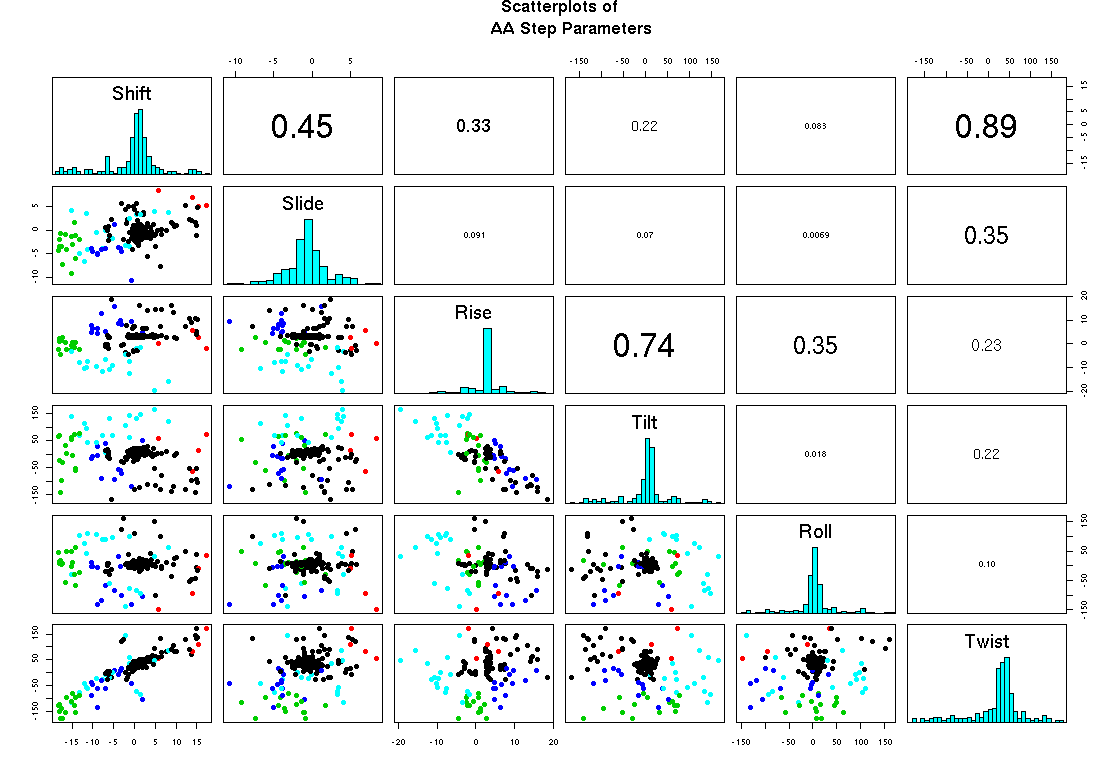
\includegraphics[angle=90, scale=0.6]{All/AA.png}
\caption{Scatterplots for step-parameters of \textbf{All} AA dinucleotide steps
in 50S rRNA.}
\label{fig:stepsAA}
\end{figure}

\begin{figure}[H]
\centering
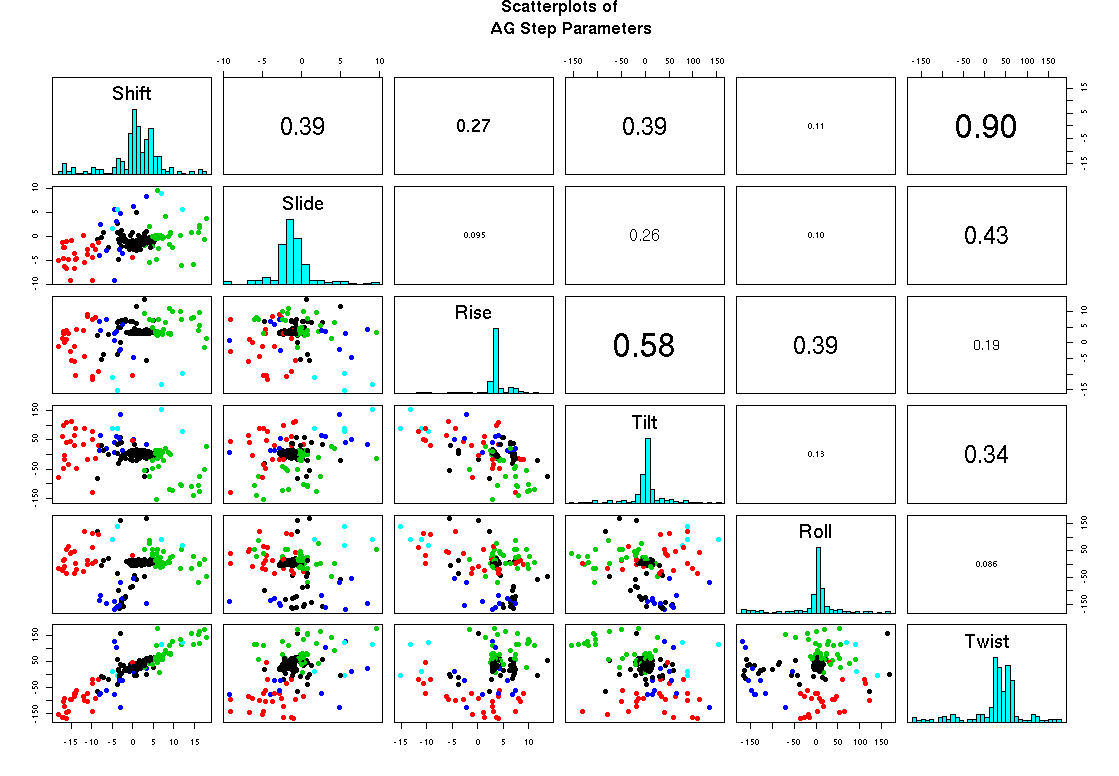
\includegraphics[angle=90, scale=0.6]{All/AG.png}
\caption{Scatterplots for step-parameters of \textbf{All} AG dinucleotide steps
in 50S rRNA.}
\label{fig:stepsAG}
\end{figure}

\begin{figure}[H]
\centering
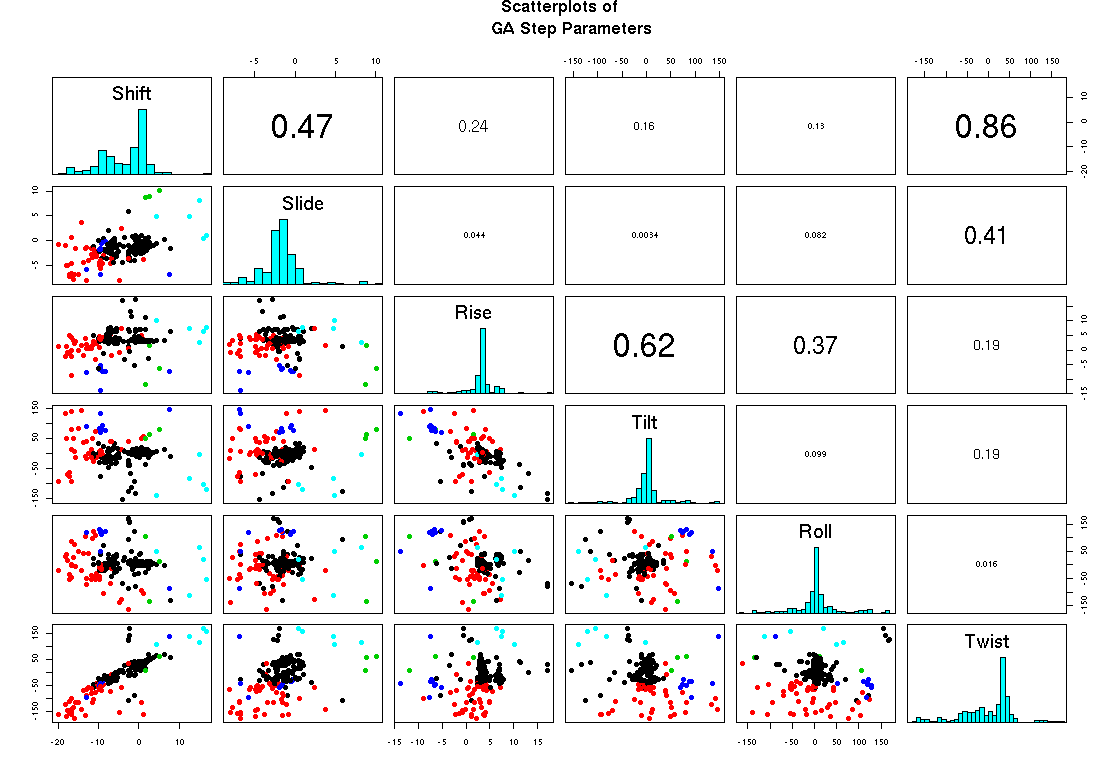
\includegraphics[angle=90, scale=0.6]{All/GA.png}
\caption{Scatterplots for step-parameters of \textbf{All} GA dinucleotide steps
in 50S rRNA.}
\label{fig:stepsGA}
\end{figure}

\begin{figure}[H]
\centering
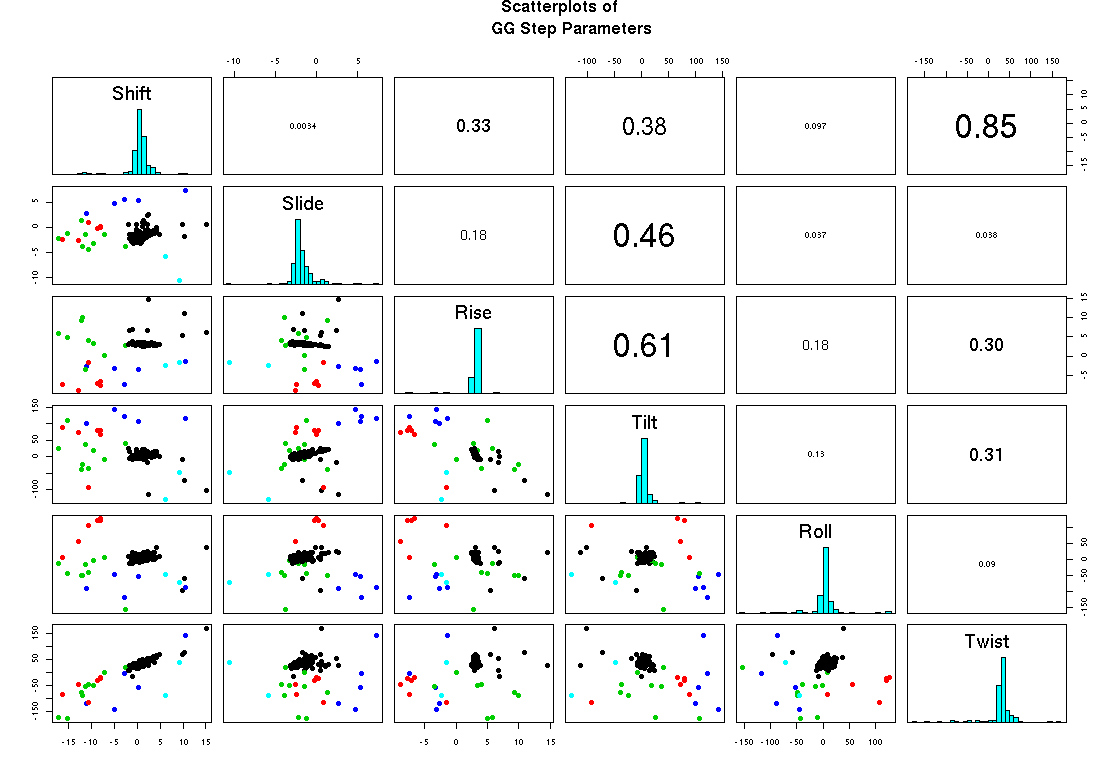
\includegraphics[angle=90, scale=0.6]{All/GG.png}
\caption{Scatterplots for step-parameters of \textbf{All} GG dinucleotide steps
in 50S rRNA.}
\label{fig:stepsGG}
\end{figure}

\begin{figure}[H]
\centering
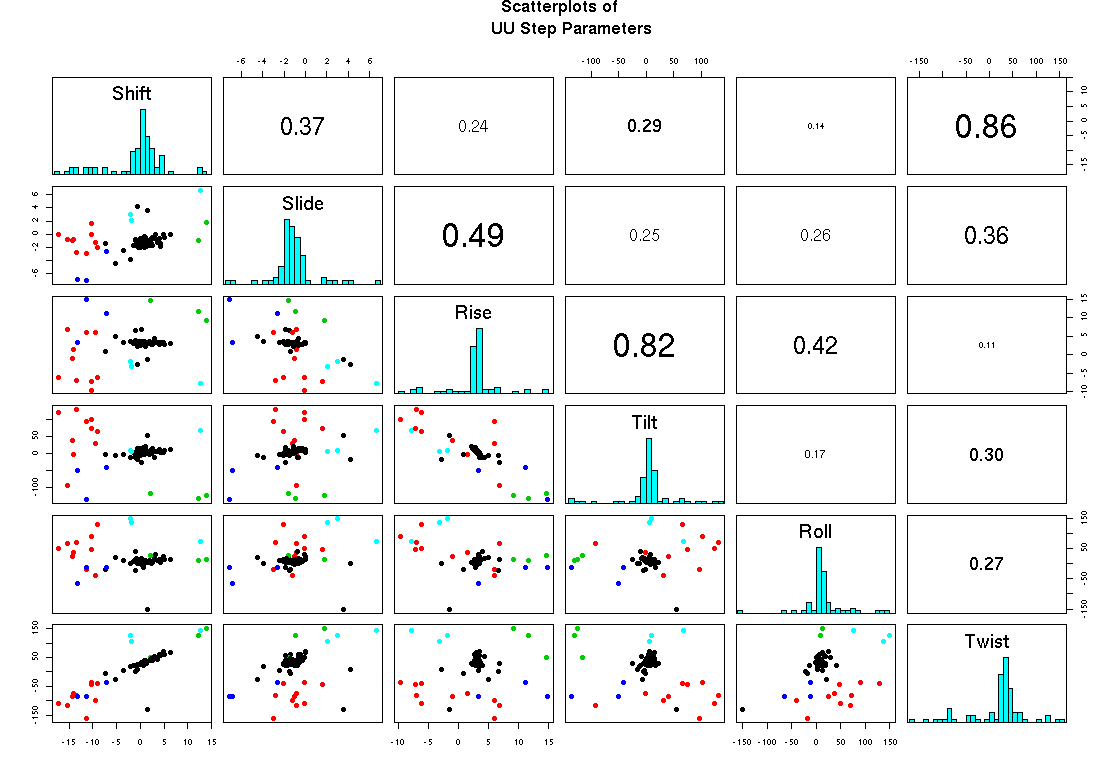
\includegraphics[angle=90, scale=0.6]{All/UU.png}
\caption{Scatterplots for step-parameters of \textbf{All} UU dinucleotide steps
in 50S rRNA.}
\label{fig:stepsUU}
\end{figure}

\begin{figure}[H]
\centering
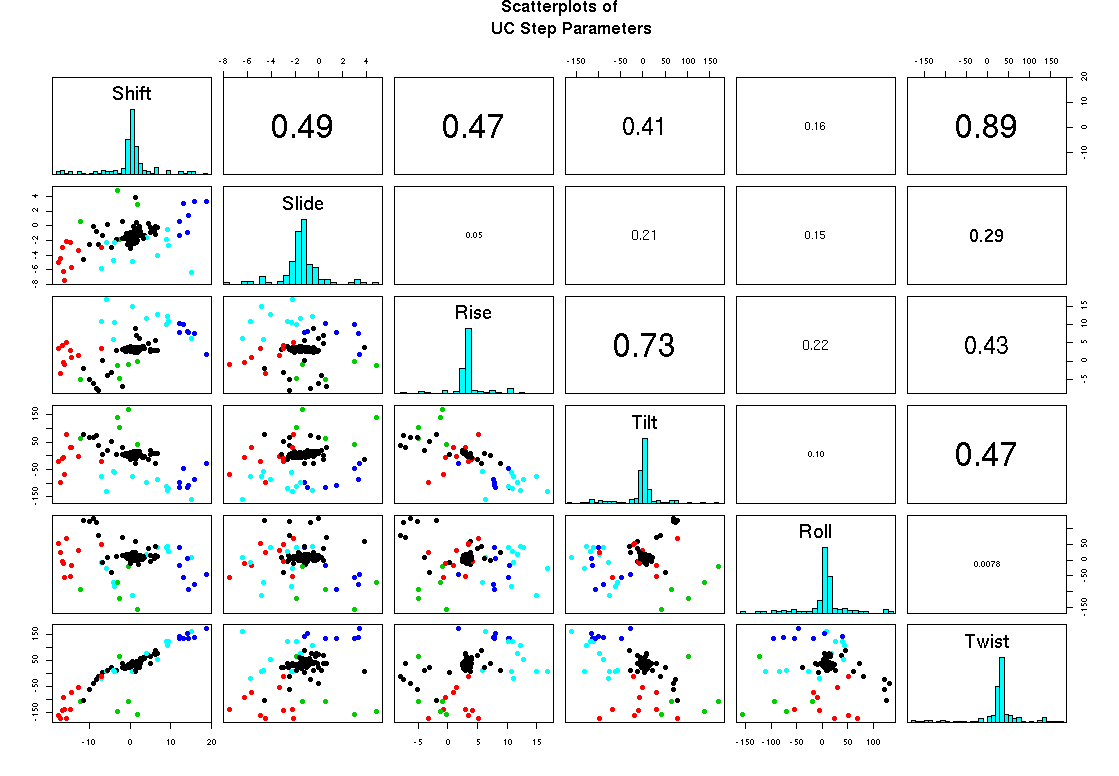
\includegraphics[angle=90, scale=0.6]{All/UC.png}
\caption{Scatterplots for step-parameters of \textbf{All} UC dinucleotide steps
in 50S rRNA.}
\label{fig:stepsUC}
\end{figure}

\begin{figure}[H]
\centering
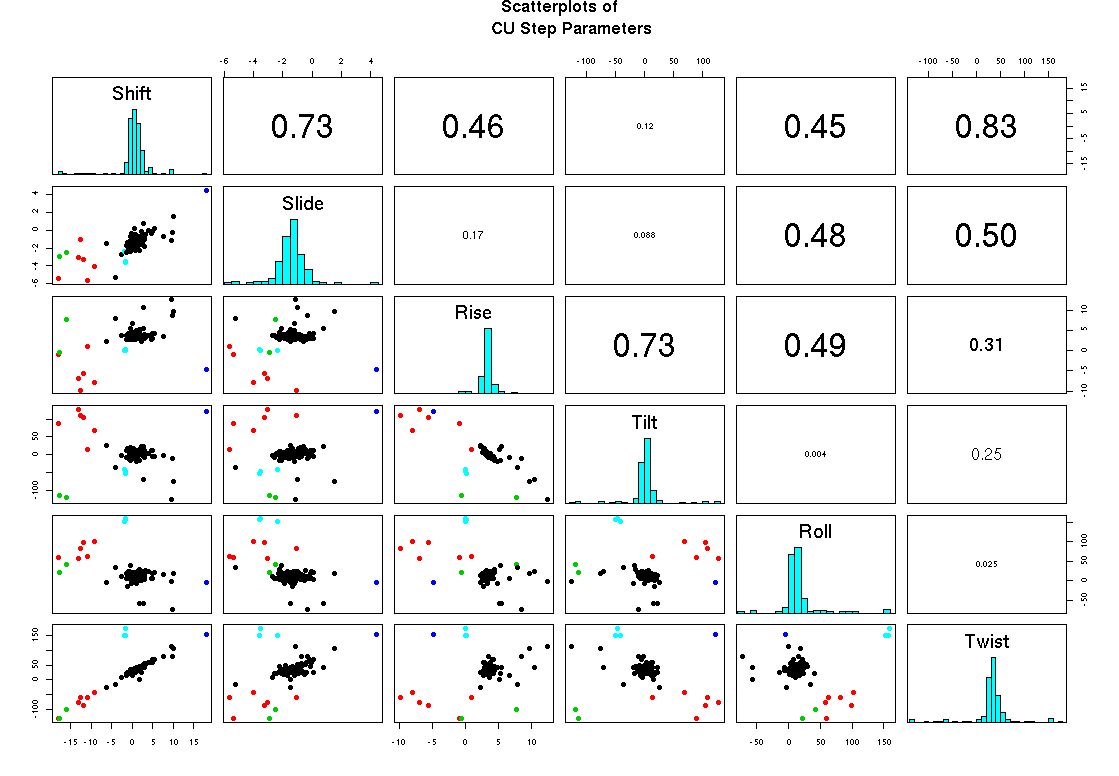
\includegraphics[angle=90, scale=0.6]{All/CU.png}
\caption{Scatterplots for step-parameters of \textbf{All} CU dinucleotide steps
in 50S rRNA.}
\label{fig:stepsCU}
\end{figure}

\begin{figure}[H]
\centering
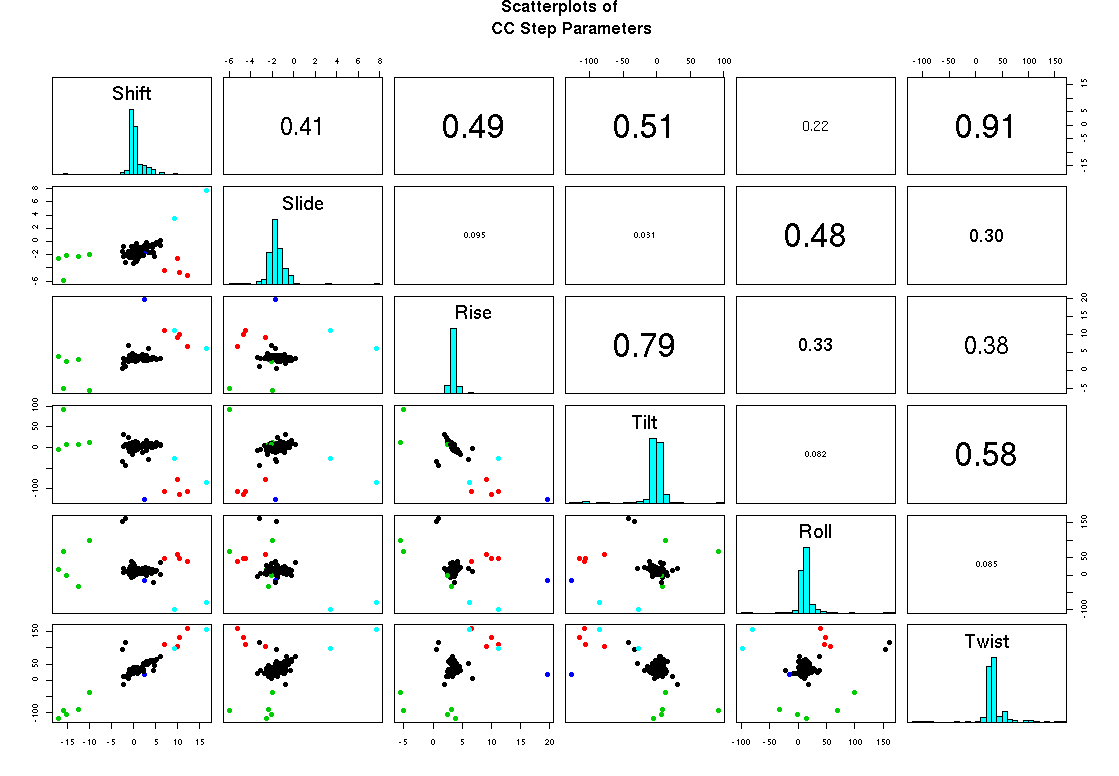
\includegraphics[angle=90, scale=0.6]{All/CC.png}
\caption{Scatterplots for step-parameters of \textbf{All} CC dinucleotide steps
in 50S rRNA.}
\label{fig:stepsCC}
\end{figure}

\begin{figure}[H]
\centering
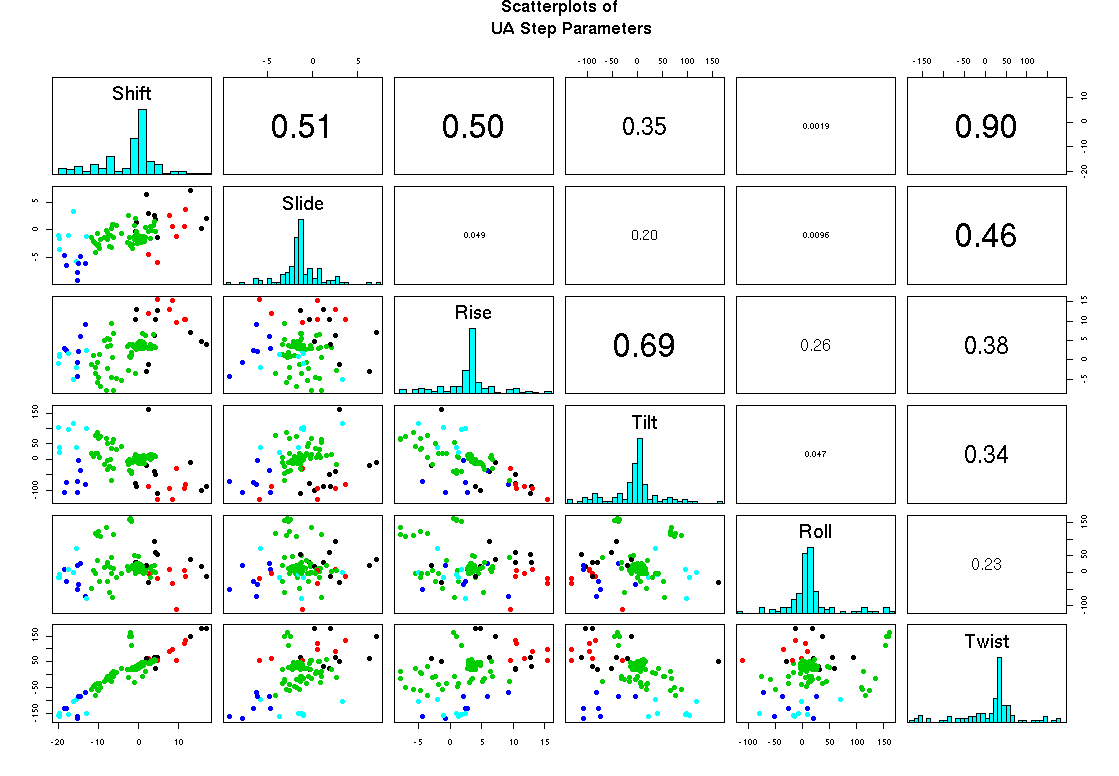
\includegraphics[angle=90, scale=0.6]{All/UA.png}
\caption{Scatterplots for step-parameters of \textbf{All} UA dinucleotide steps
in 50S rRNA.}
\label{fig:stepsUA}
\end{figure}

\begin{figure}[H]
\centering
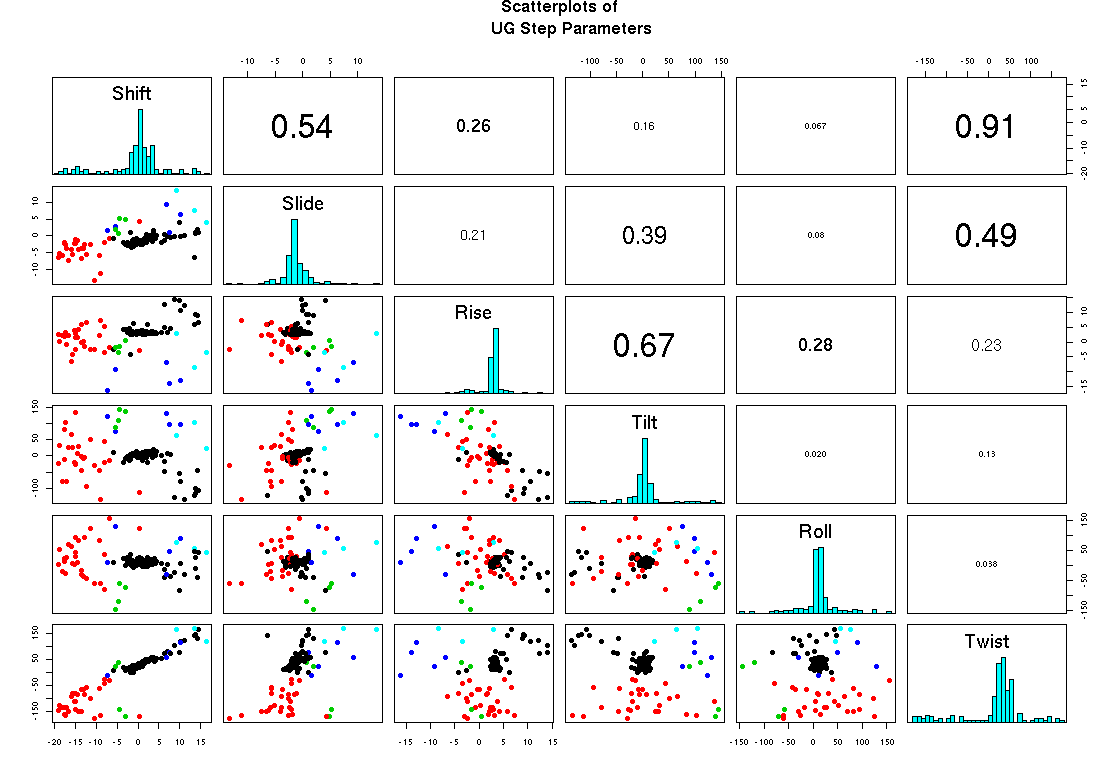
\includegraphics[angle=90, scale=0.6]{All/UG.png}
\caption{Scatterplots for step-parameters of \textbf{All} UG dinucleotide steps
in 50S rRNA.}
\label{fig:stepsUG}
\end{figure}

\begin{figure}[H]
\centering
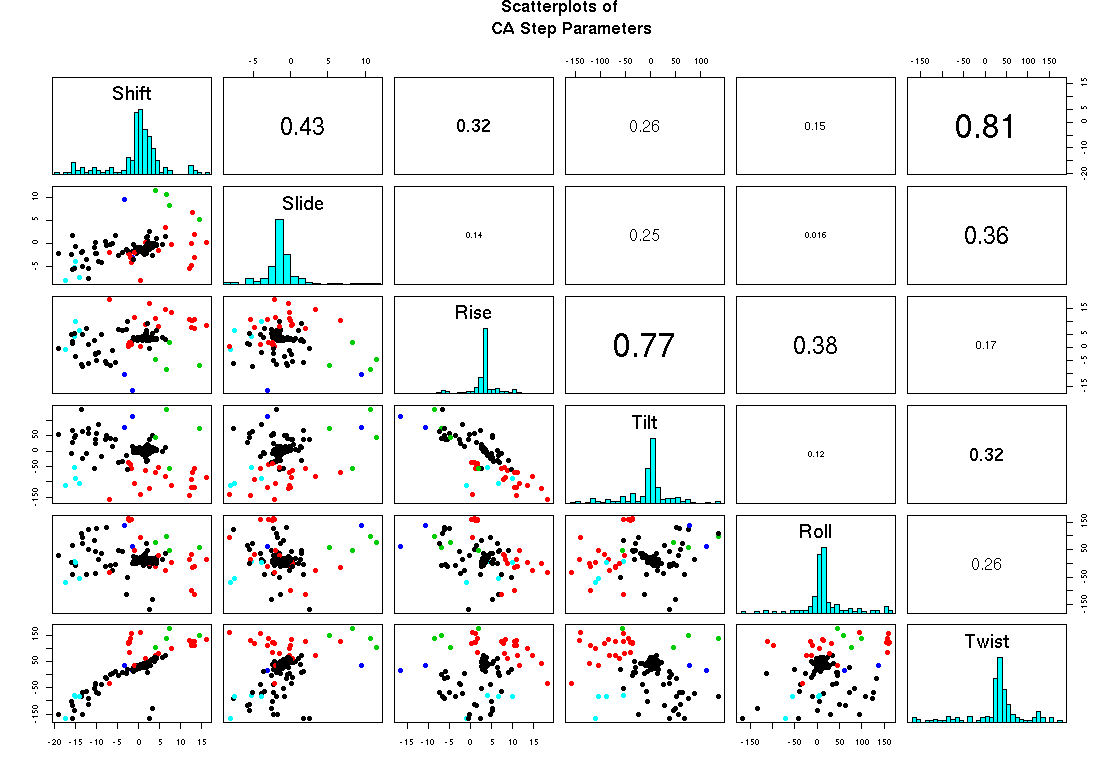
\includegraphics[angle=90, scale=0.6]{All/CA.png}
\caption{Scatterplots for step-parameters of \textbf{All} CA dinucleotide steps
in 50S rRNA.}
\label{fig:stepsCA}
\end{figure}

\begin{figure}[H]
\centering
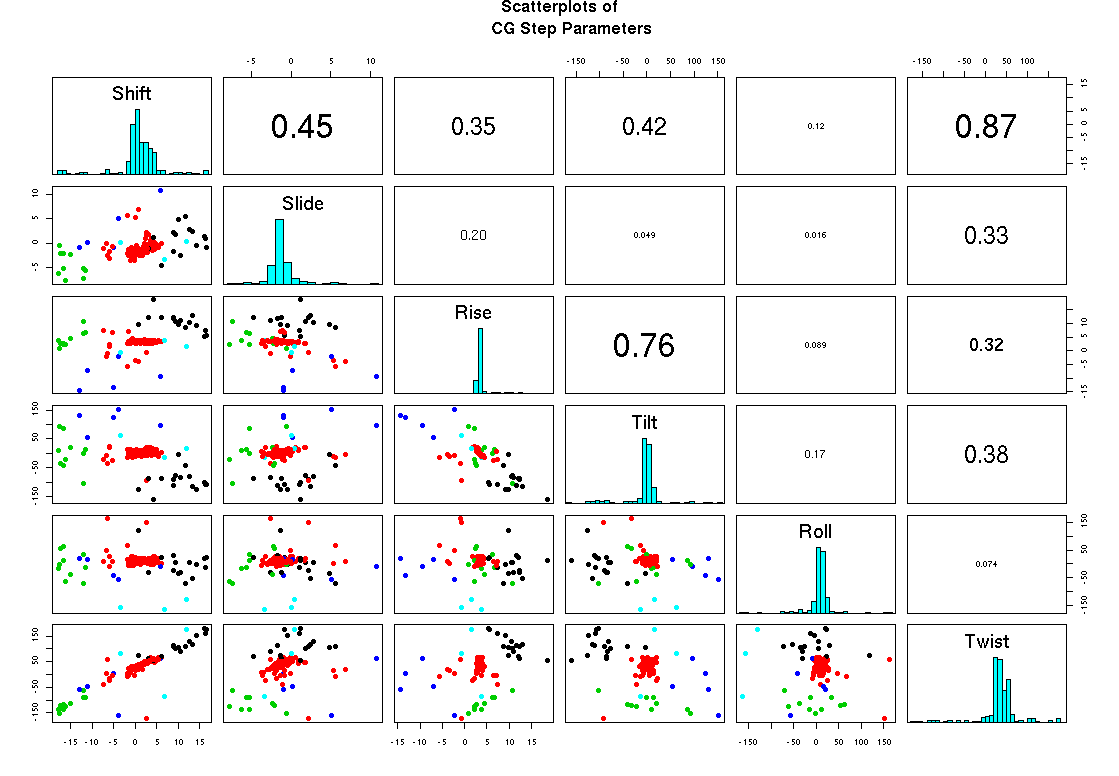
\includegraphics[angle=90, scale=0.6]{All/CG.png}
\caption{Scatterplots for step-parameters of \textbf{All} CG dinucleotide steps
in 50S rRNA.}
\label{fig:stepsCG}
\end{figure}

\begin{figure}[H]
\centering
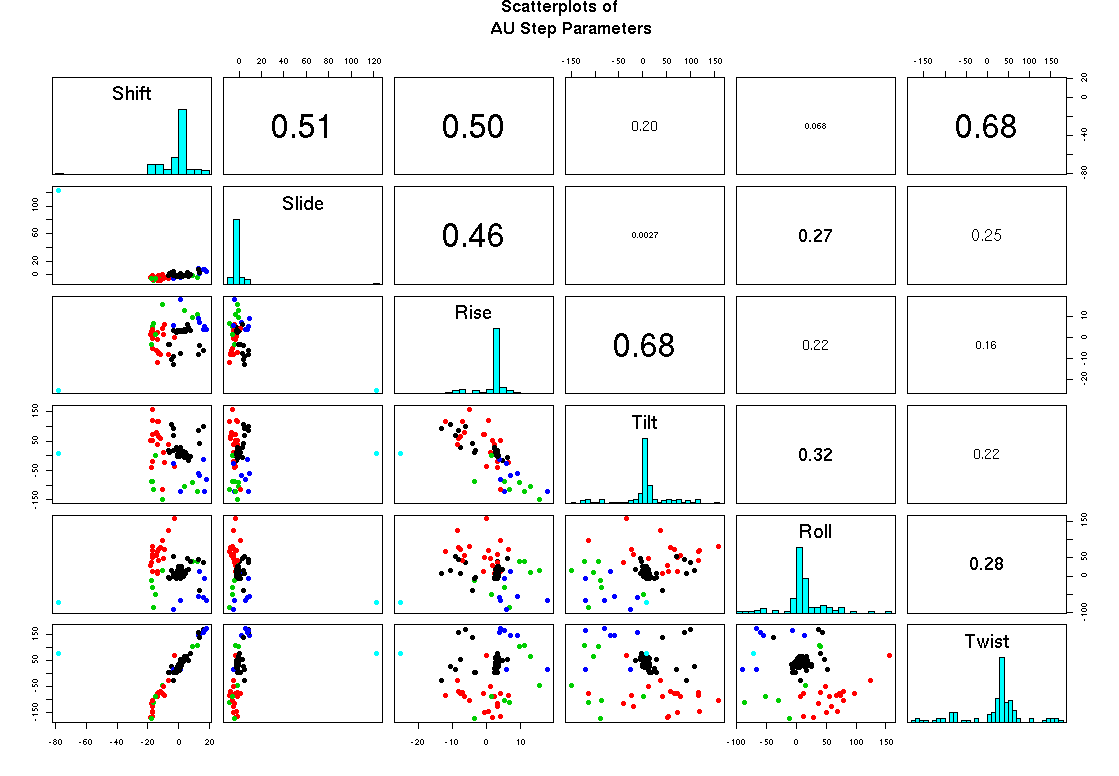
\includegraphics[angle=90, scale=0.6]{All/AU.png}
\caption{Scatterplots for step-parameters of \textbf{All} AU dinucleotide steps
in 50S rRNA.}
\label{fig:stepsAU}
\end{figure}

\begin{figure}[H]
\centering
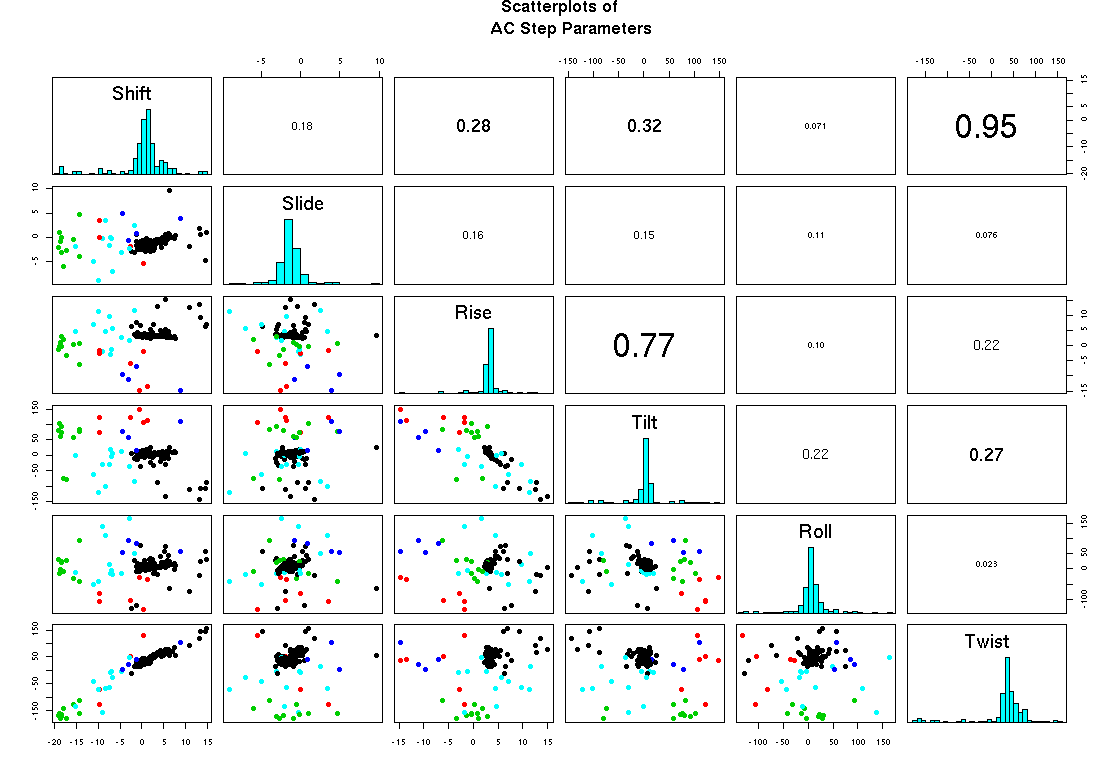
\includegraphics[angle=90, scale=0.6]{All/AC.png}
\caption{Scatterplots for step-parameters of \textbf{All} AC dinucleotide steps
in 50S rRNA.}
\label{fig:stepsAC}
\end{figure}

\begin{figure}[H]
\centering
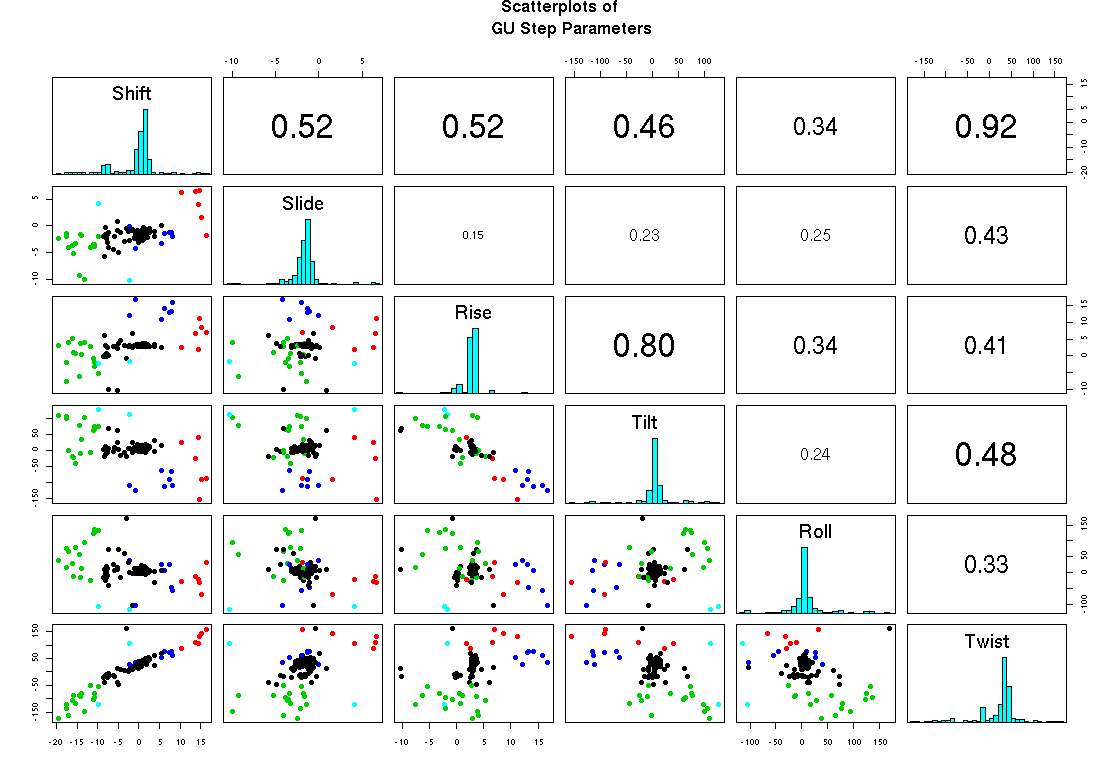
\includegraphics[angle=90, scale=0.6]{All/GU.png}
\caption{Scatterplots for step-parameters of \textbf{All} GU dinucleotide steps
in 50S rRNA.}
\label{fig:stepsGU}
\end{figure}

\begin{figure}[H]
\centering
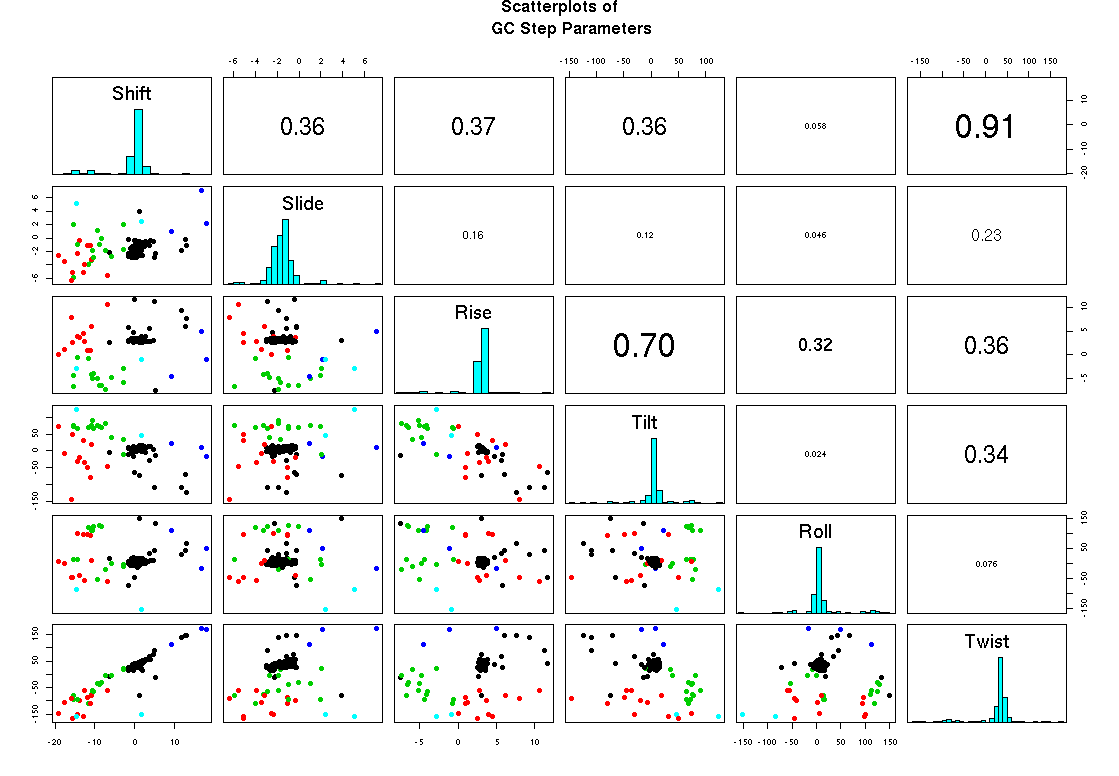
\includegraphics[angle=90, scale=0.6]{All/GC.png}
\caption{Scatterplots for step-parameters of \textbf{All} GC dinucleotide steps
in 50S rRNA.}
\label{fig:stepsGC}
\end{figure}

%%%%%%%%%%%%%%%%%%%%%%%%%%%%%%%%%%%%%%%%%%%%%%%%%
%THE FOLLOWING ARE THE SCATTERPLOTS FOR HELICAL STEPS
%%%%%%%%%%%%%%%%%%%%%%%%%%%%%%%%%%%%%%%%%%%%%%%%

\begin{figure}[H]
\centering
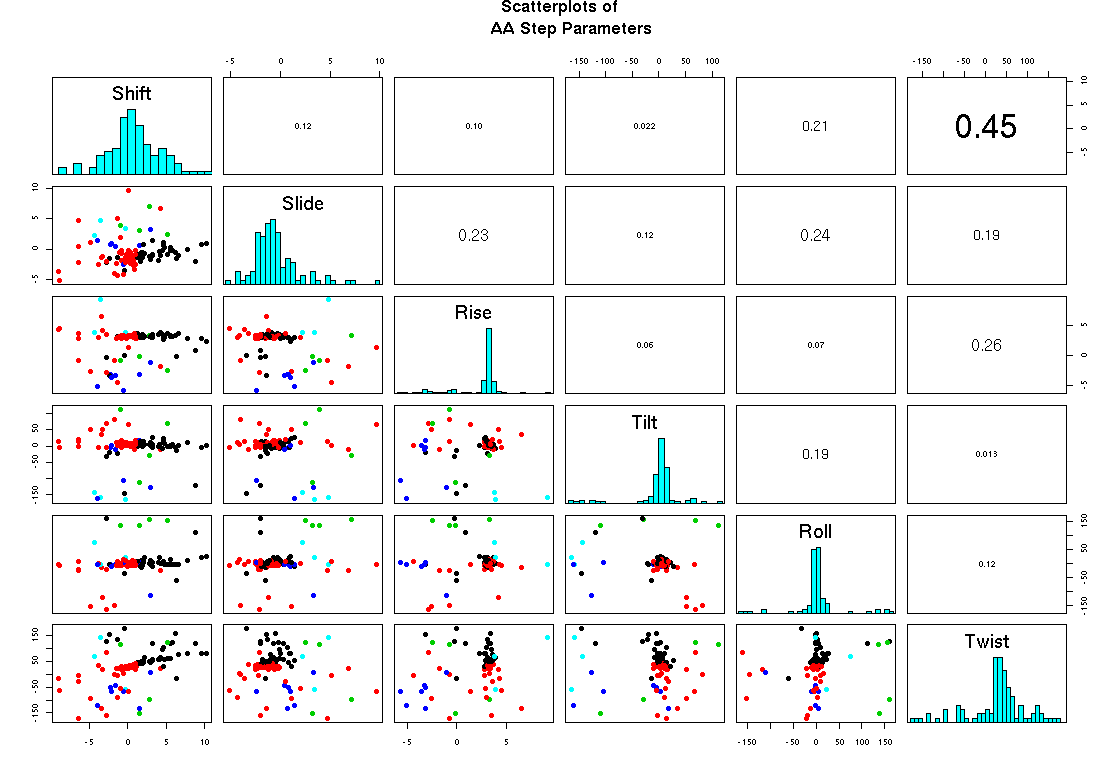
\includegraphics[angle=90, scale=0.6]{Helical/AA.png}
\caption{Scatterplots for step-parameters of \textbf{Helical} AA dinucleotide steps
in 50S rRNA.}
\label{fig:stepsAA}
\end{figure}

\begin{figure}[H]
\centering
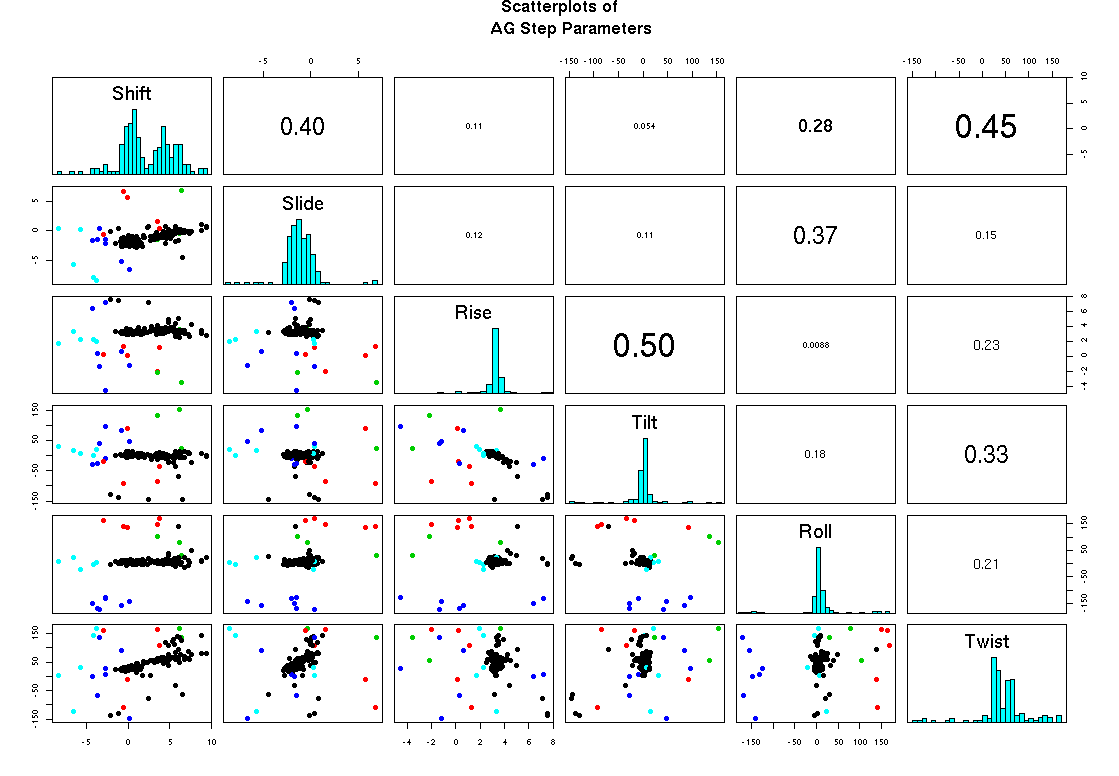
\includegraphics[angle=90, scale=0.6]{Helical/AG.png}
\caption{Scatterplots for step-parameters of \textbf{Helical} AG dinucleotide steps
in 50S rRNA.}
\label{fig:stepsAG}
\end{figure}

\begin{figure}[H]
\centering
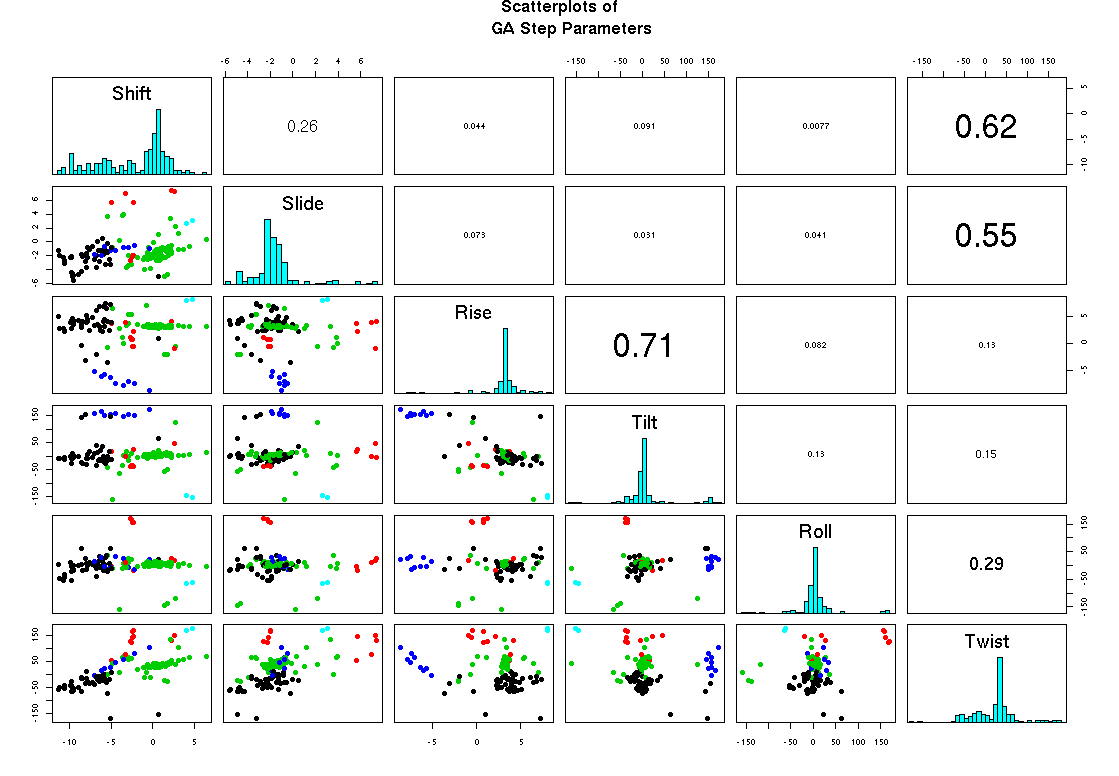
\includegraphics[angle=90, scale=0.6]{Helical/GA.png}
\caption{Scatterplots for step-parameters of \textbf{Helical} GA dinucleotide steps
in 50S rRNA.}
\label{fig:stepsGA}
\end{figure}

\begin{figure}[H]
\centering
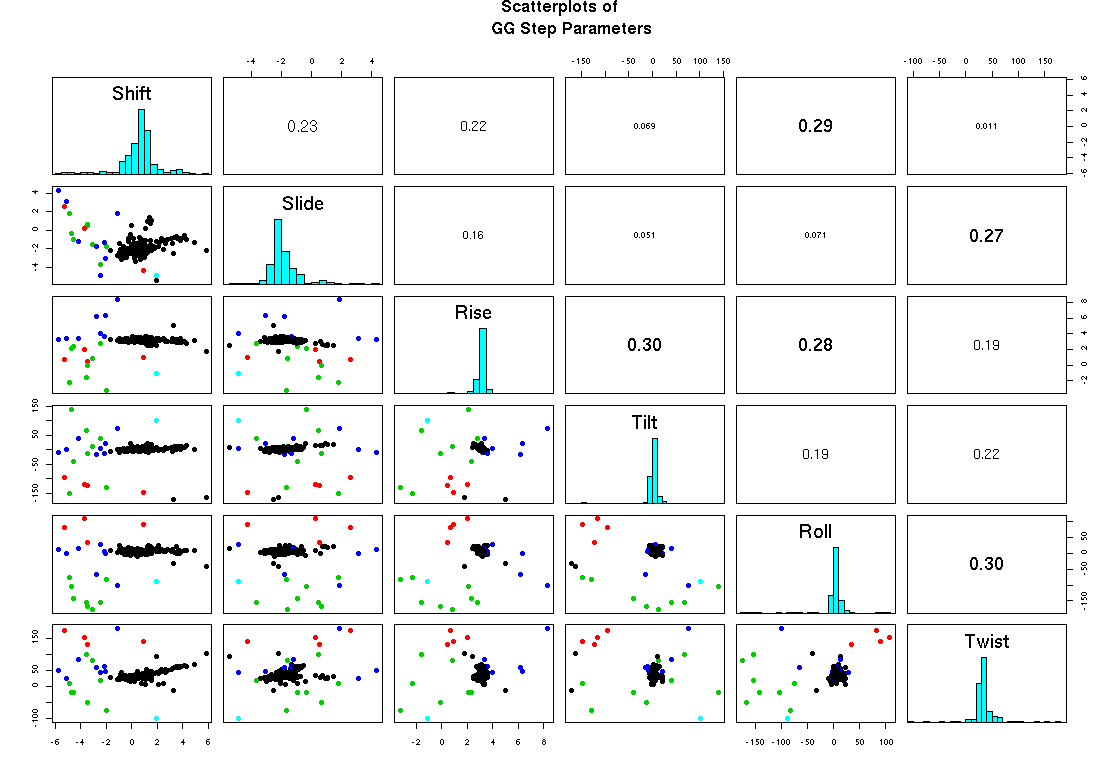
\includegraphics[angle=90, scale=0.6]{Helical/GG.png}
\caption{Scatterplots for step-parameters of \textbf{Helical} GG dinucleotide steps
in 50S rRNA.}
\label{fig:stepsGG}
\end{figure}

\begin{figure}[H]
\centering
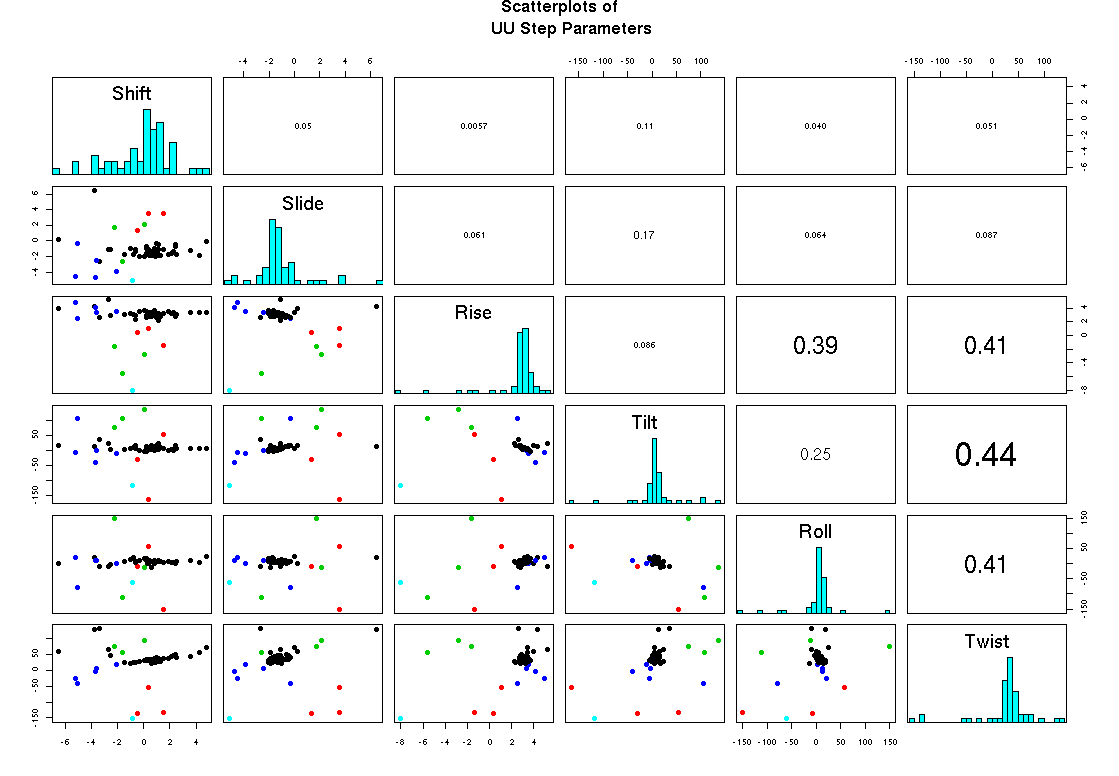
\includegraphics[angle=90, scale=0.6]{Helical/UU.png}
\caption{Scatterplots for step-parameters of \textbf{Helical} UU dinucleotide steps
in 50S rRNA.}
\label{fig:stepsUU}
\end{figure}

\begin{figure}[H]
\centering
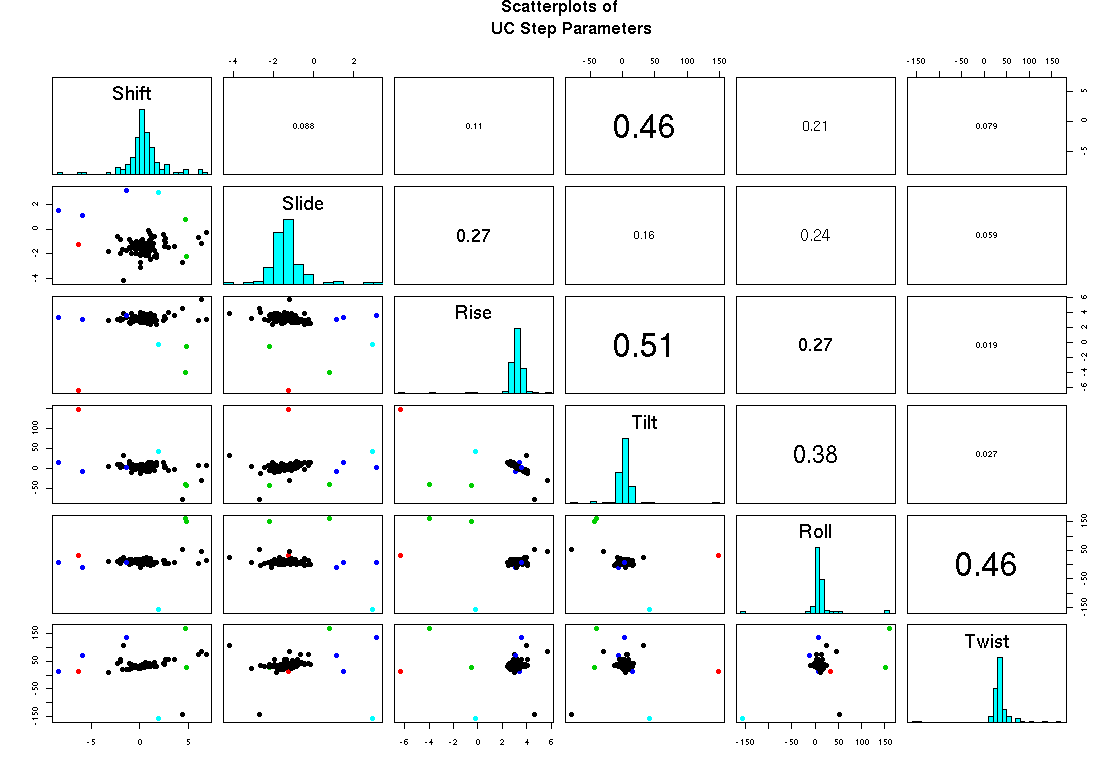
\includegraphics[angle=90, scale=0.6]{Helical/UC.png}
\caption{Scatterplots for step-parameters of \textbf{Helical} UC dinucleotide steps
in 50S rRNA.}
\label{fig:stepsUC}
\end{figure}

\begin{figure}[H]
\centering
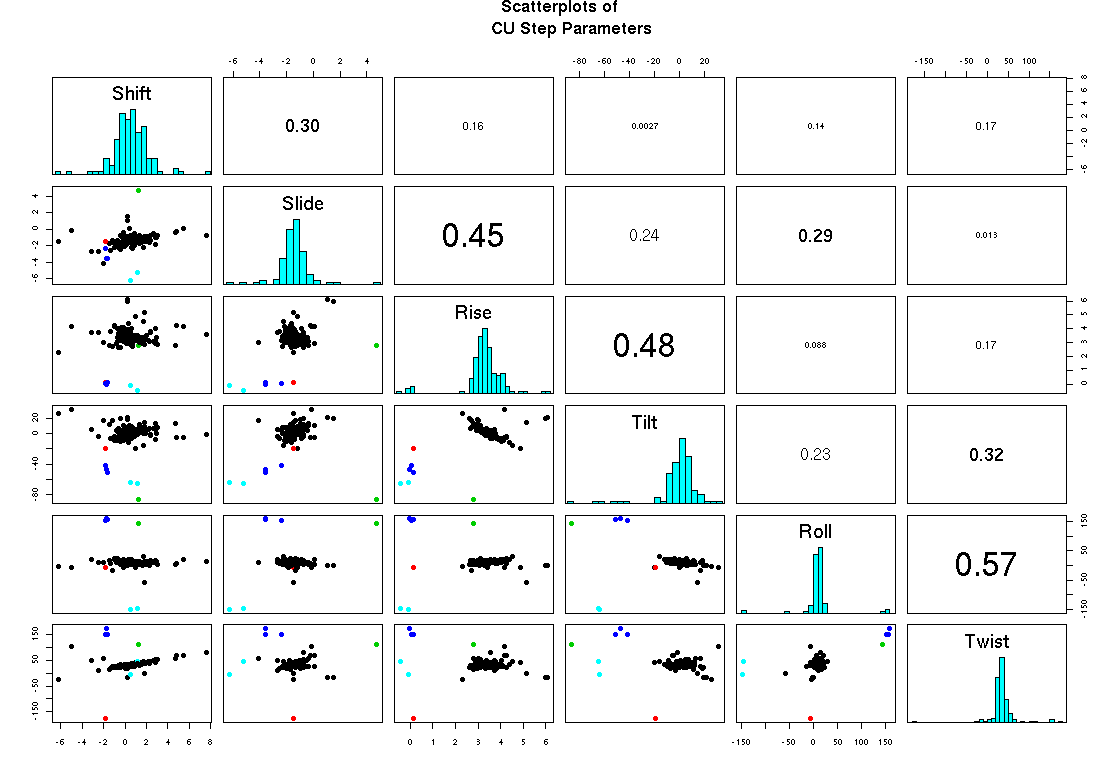
\includegraphics[angle=90, scale=0.6]{Helical/CU.png}
\caption{Scatterplots for step-parameters of \textbf{Helical} CU dinucleotide steps
in 50S rRNA.}
\label{fig:stepsCU}
\end{figure}

\begin{figure}[H]
\centering
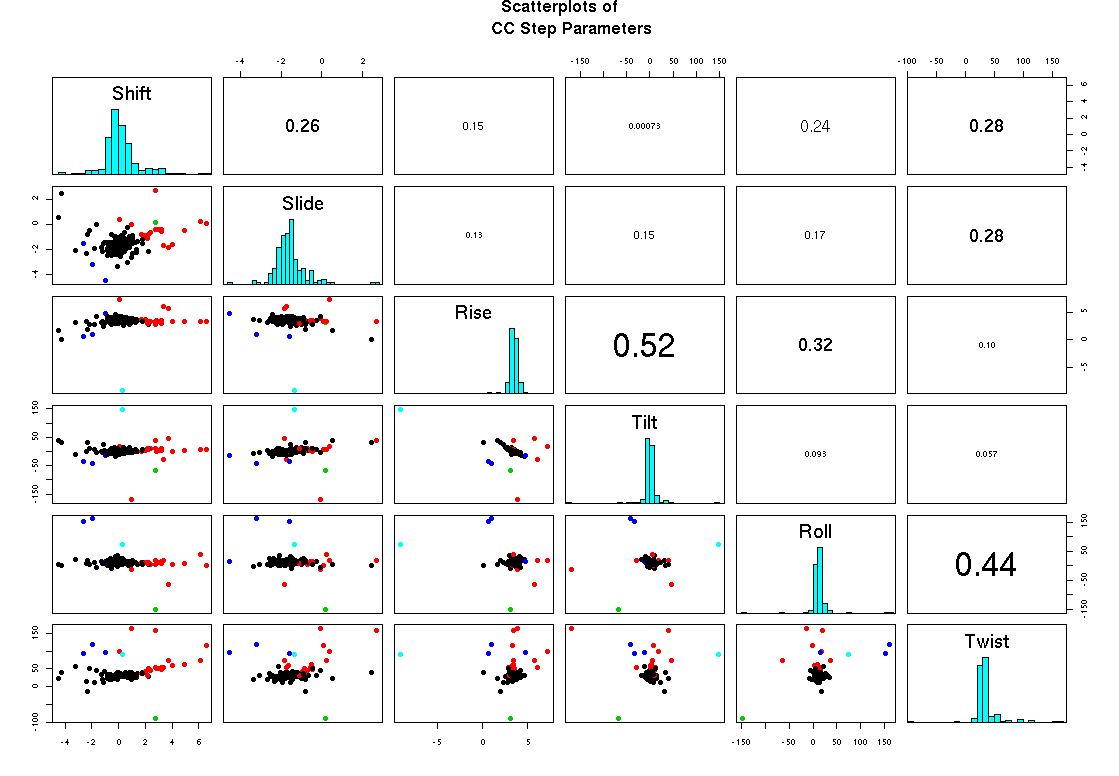
\includegraphics[angle=90, scale=0.6]{Helical/CC.png}
\caption{Scatterplots for step-parameters of \textbf{Helical} CC dinucleotide steps
in 50S rRNA.}
\label{fig:stepsCC}
\end{figure}

\begin{figure}[H]
\centering
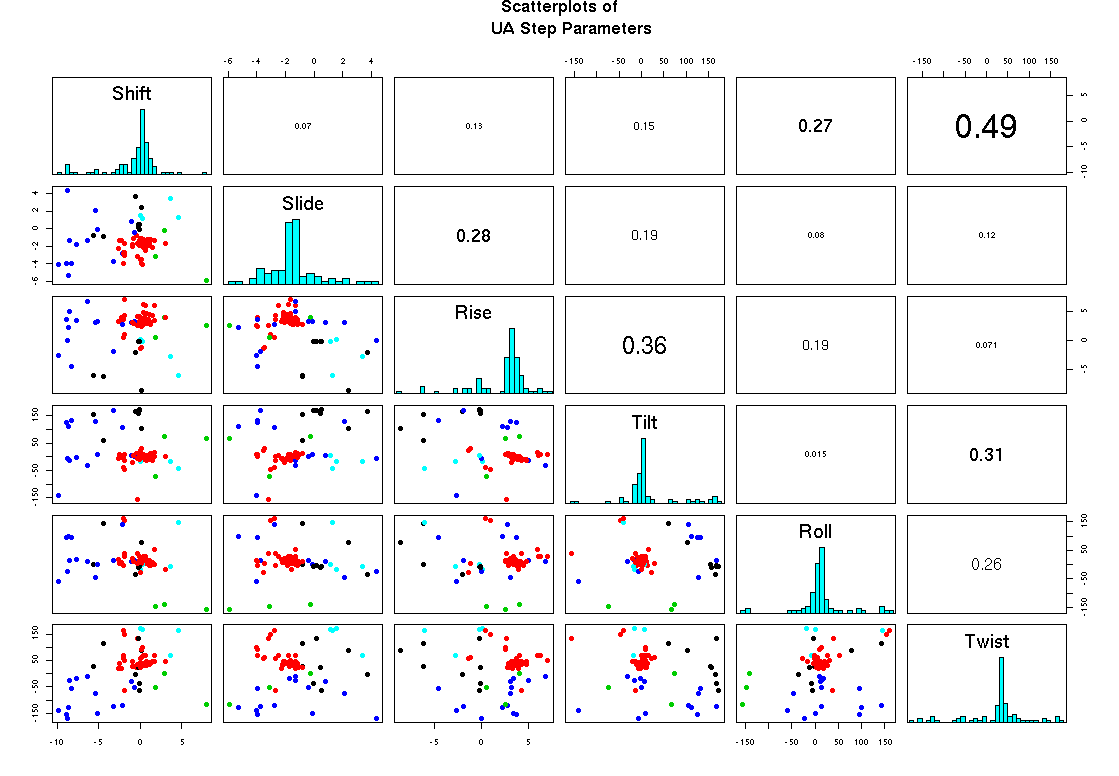
\includegraphics[angle=90, scale=0.6]{Helical/UA.png}
\caption{Scatterplots for step-parameters of \textbf{Helical} UA dinucleotide steps
in 50S rRNA.}
\label{fig:stepsUA}
\end{figure}

\begin{figure}[H]
\centering
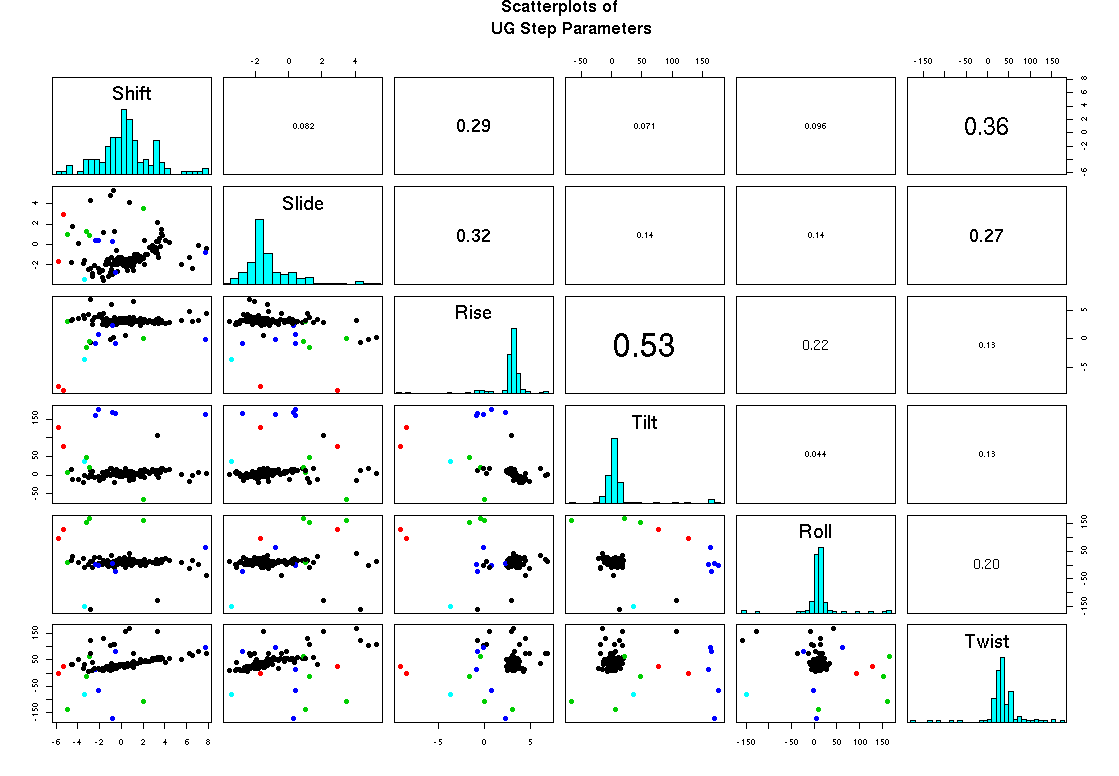
\includegraphics[angle=90, scale=0.6]{Helical/UG.png}
\caption{Scatterplots for step-parameters of \textbf{Helical} UG dinucleotide steps
in 50S rRNA.}
\label{fig:stepsUG}
\end{figure}

\begin{figure}[H]
\centering
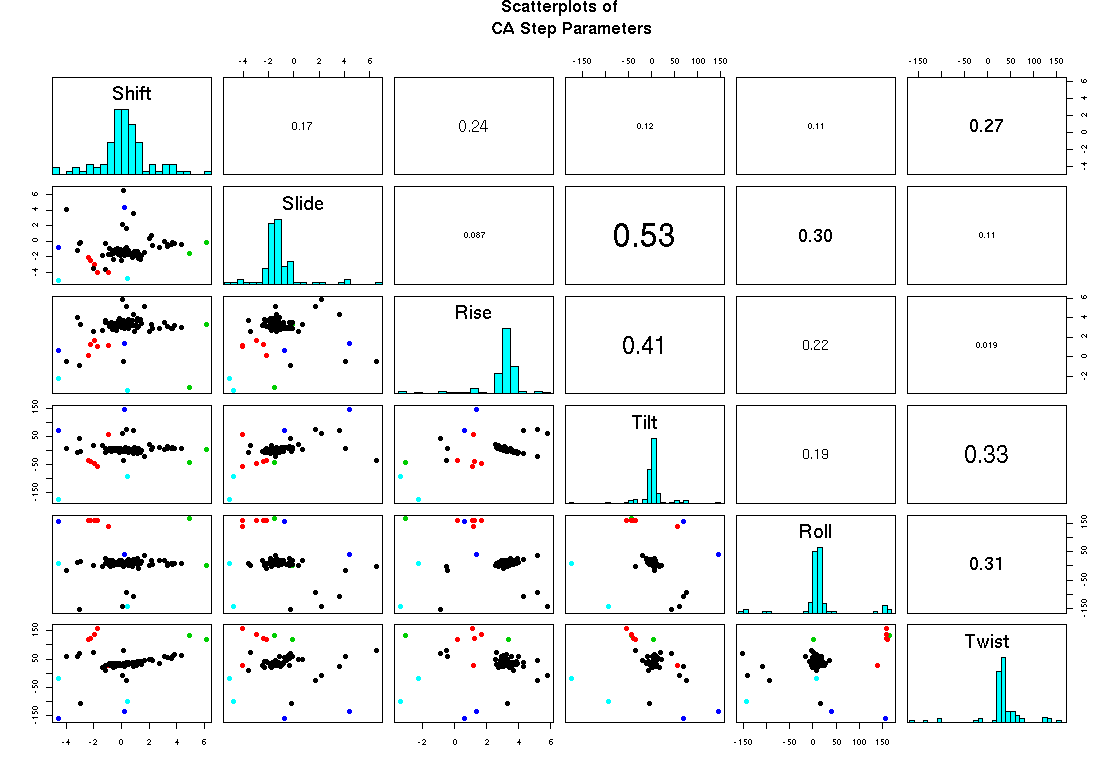
\includegraphics[angle=90, scale=0.6]{Helical/CA.png}
\caption{Scatterplots for step-parameters of \textbf{Helical} CA dinucleotide steps
in 50S rRNA.}
\label{fig:stepsCA}
\end{figure}

\begin{figure}[H]
\centering
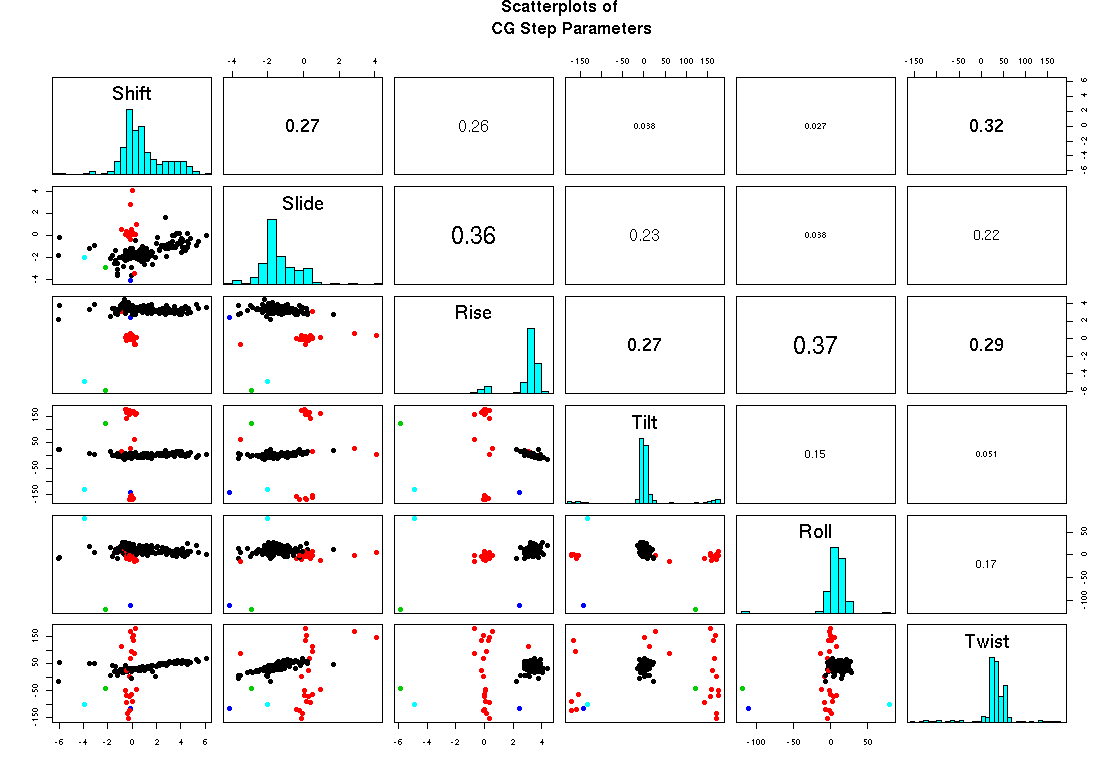
\includegraphics[angle=90, scale=0.6]{Helical/CG.png}
\caption{Scatterplots for step-parameters of \textbf{Helical} CG dinucleotide steps
in 50S rRNA.}
\label{fig:stepsCG}
\end{figure}

\begin{figure}[H]
\centering
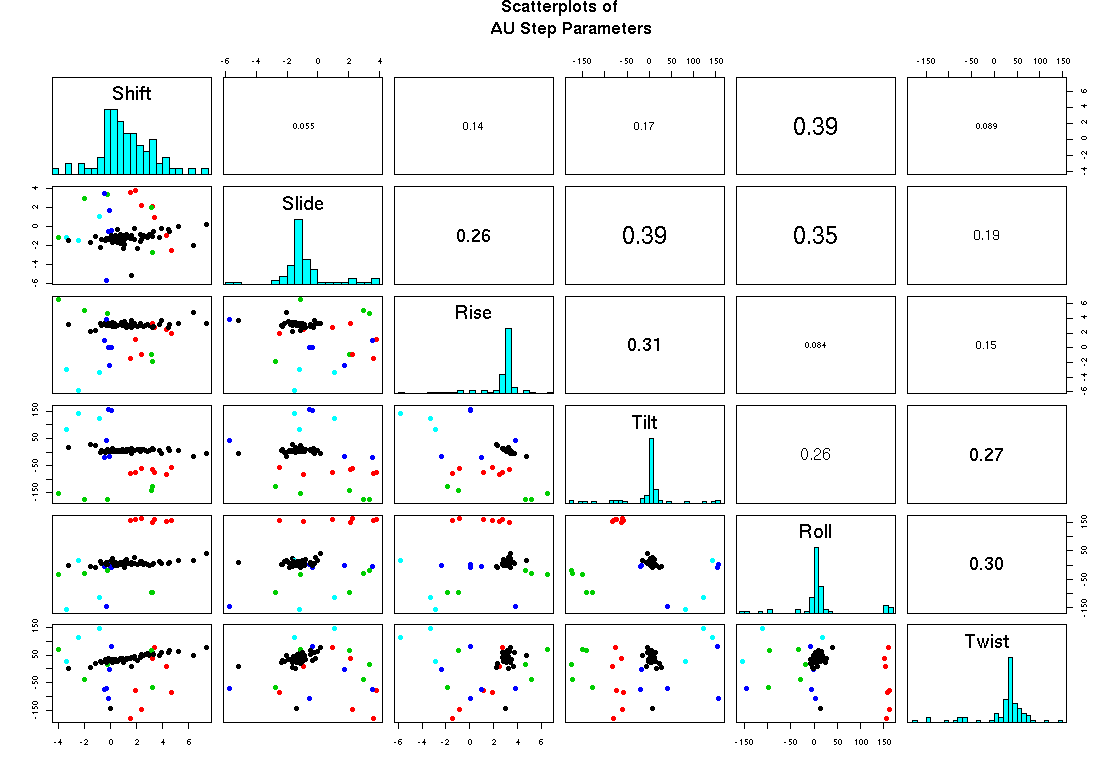
\includegraphics[angle=90, scale=0.6]{Helical/AU.png}
\caption{Scatterplots for step-parameters of \textbf{Helical} AU dinucleotide steps
in 50S rRNA.}
\label{fig:stepsAU}
\end{figure}

\begin{figure}[H]
\centering
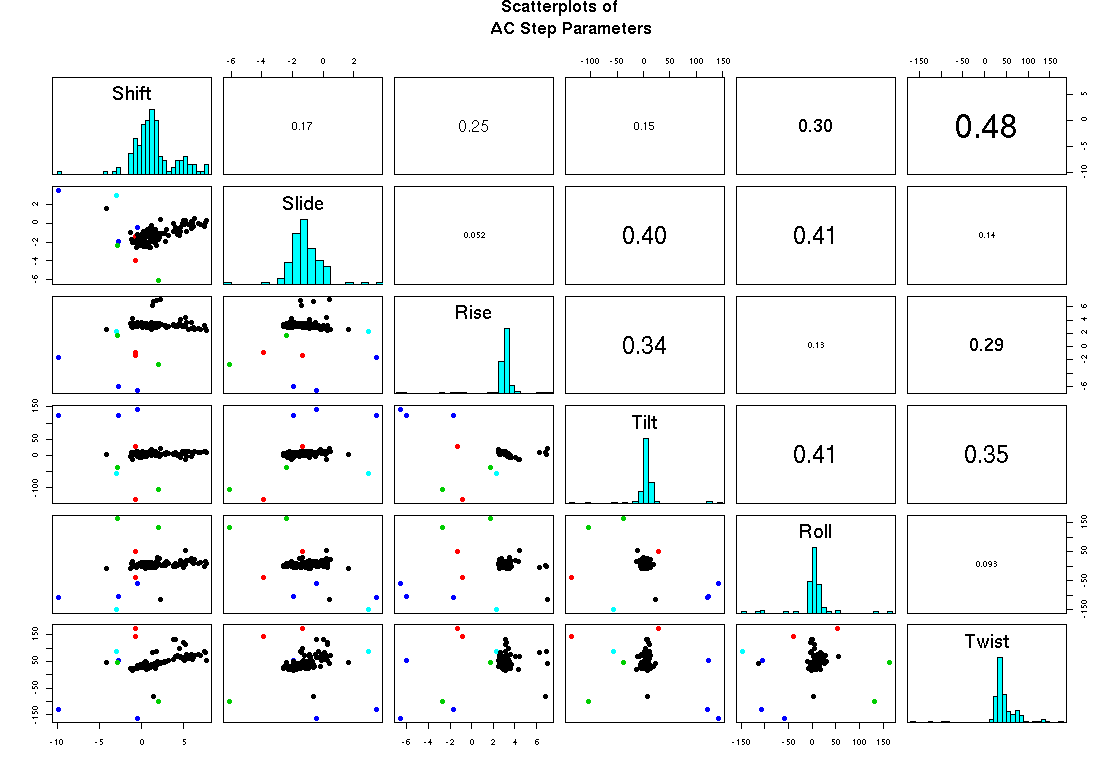
\includegraphics[angle=90, scale=0.6]{Helical/AC.png}
\caption{Scatterplots for step-parameters of \textbf{Helical} AC dinucleotide steps
in 50S rRNA.}
\label{fig:stepsAC}
\end{figure}

\begin{figure}[H]
\centering
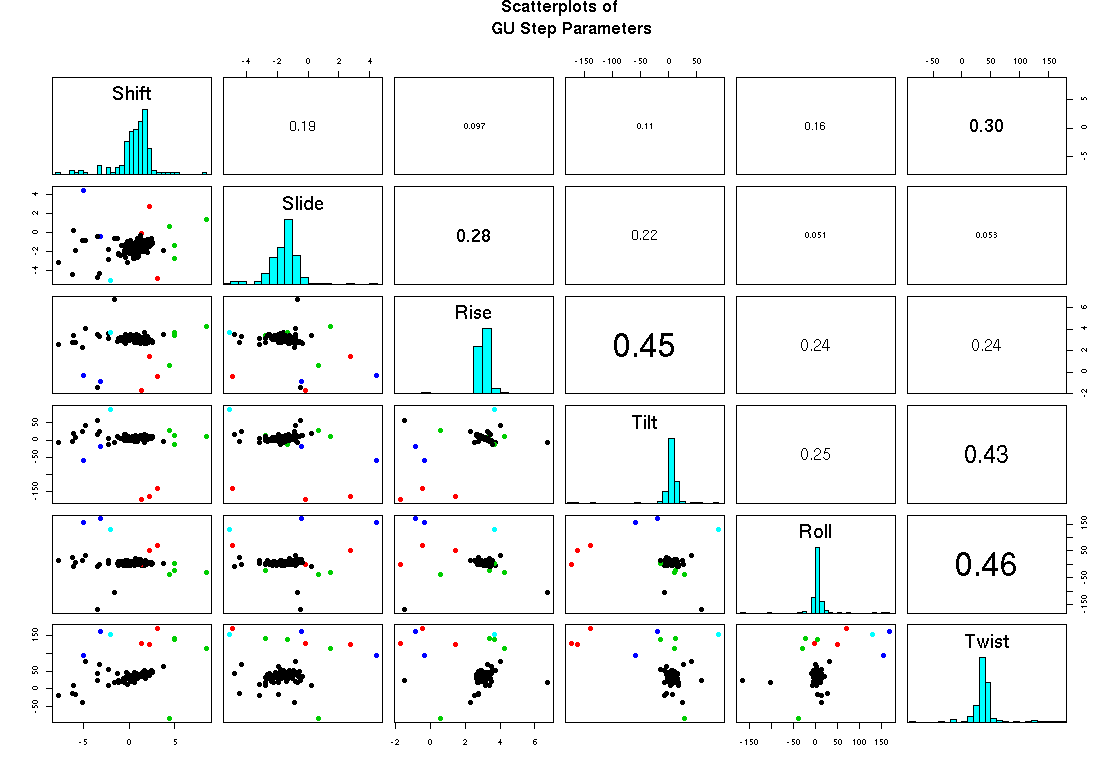
\includegraphics[angle=90, scale=0.6]{Helical/GU.png}
\caption{Scatterplots for step-parameters of \textbf{Helical} GU dinucleotide steps
in 50S rRNA.}
\label{fig:stepsGU}
\end{figure}

\begin{figure}[H]
\centering
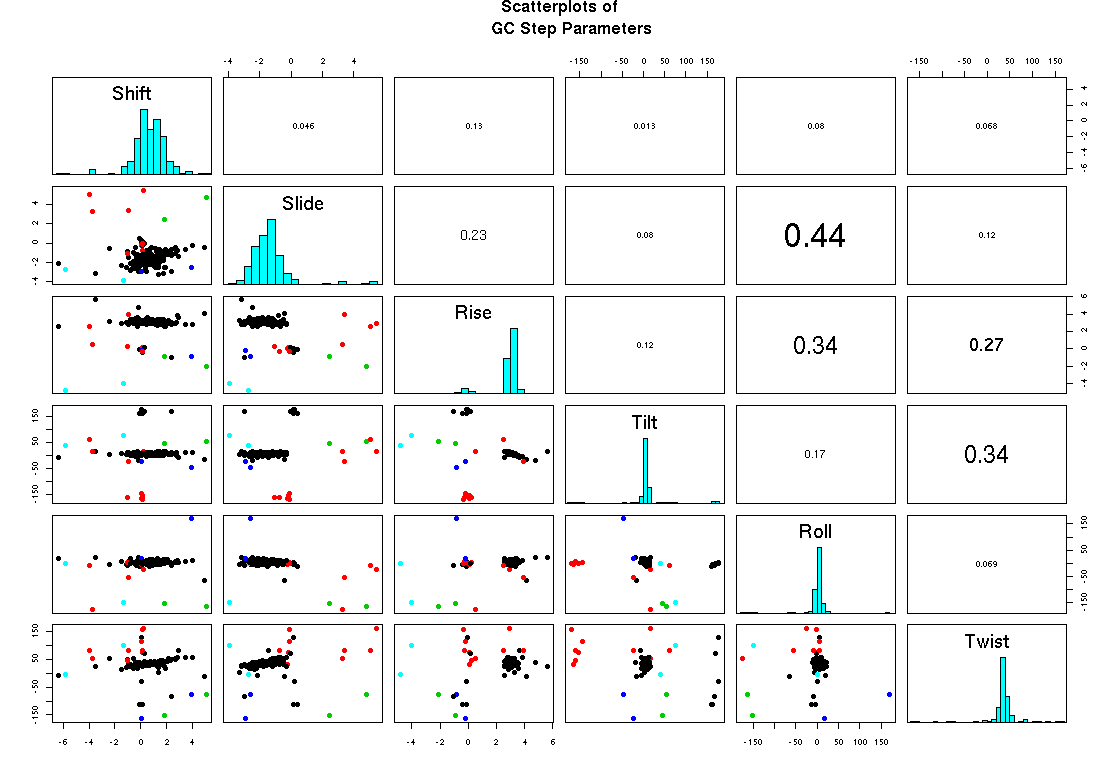
\includegraphics[angle=90, scale=0.6]{Helical/GC.png}
\caption{Scatterplots for step-parameters of \textbf{Helical} GC dinucleotide steps
in 50S rRNA.}
\label{fig:stepsGC}
\end{figure}

%%%%%%%%%%%%%%%%%%%%%%%%%%%%%%%%%%%%%%%%%%%%%%%%%
%THE FOLLOWING ARE THE SCATTERPLOTS FOR WC STEPS
%%%%%%%%%%%%%%%%%%%%%%%%%%%%%%%%%%%%%%%%%%%%%%%%

\begin{figure}[H]
\centering
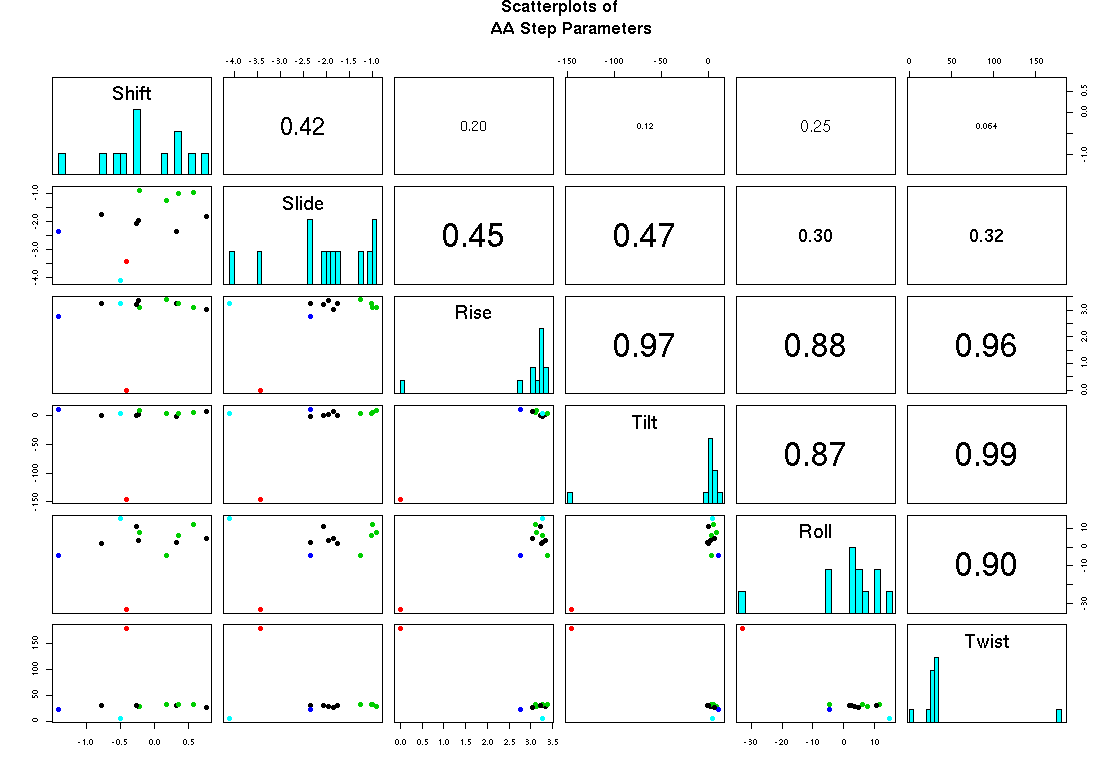
\includegraphics[angle=90, scale=0.6]{WC/AA.png}
\caption{Scatterplots for step-parameters of \textbf{WC} AA dinucleotide steps
in 50S rRNA.}
\label{fig:stepsAA}
\end{figure}

\begin{figure}[H]
\centering
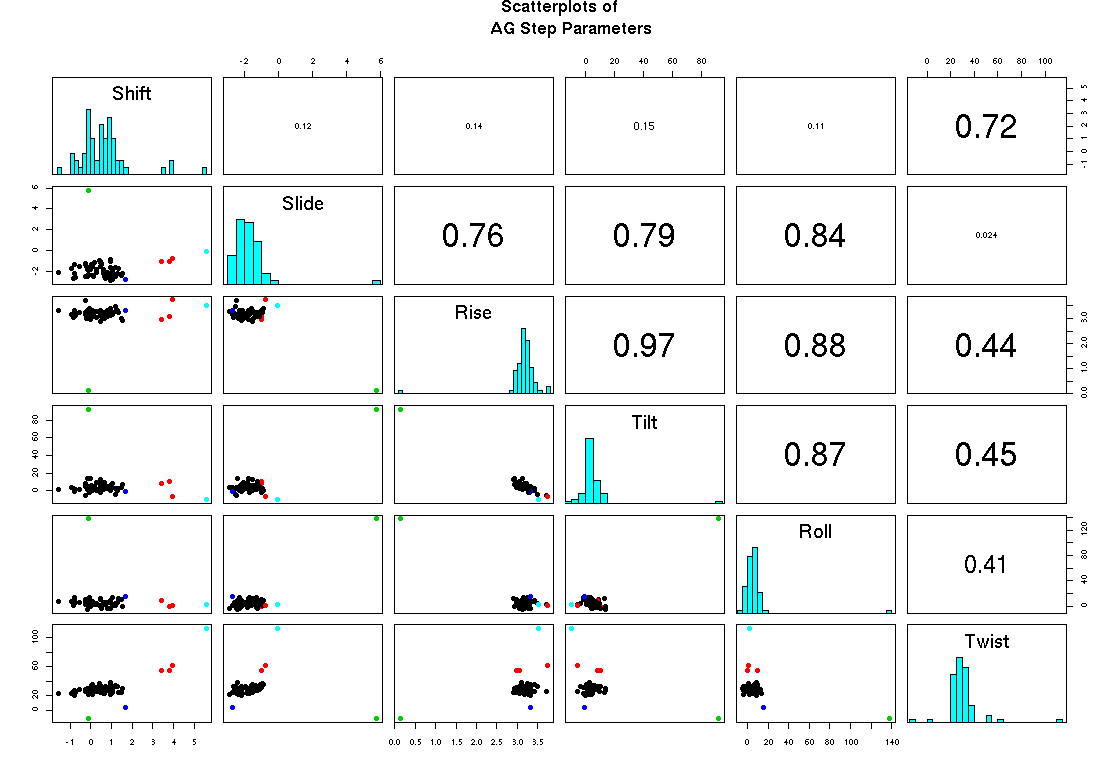
\includegraphics[angle=90, scale=0.6]{WC/AG.png}
\caption{Scatterplots for step-parameters of \textbf{WC} AG dinucleotide steps
in 50S rRNA.}
\label{fig:stepsAG}
\end{figure}

\begin{figure}[H]
\centering
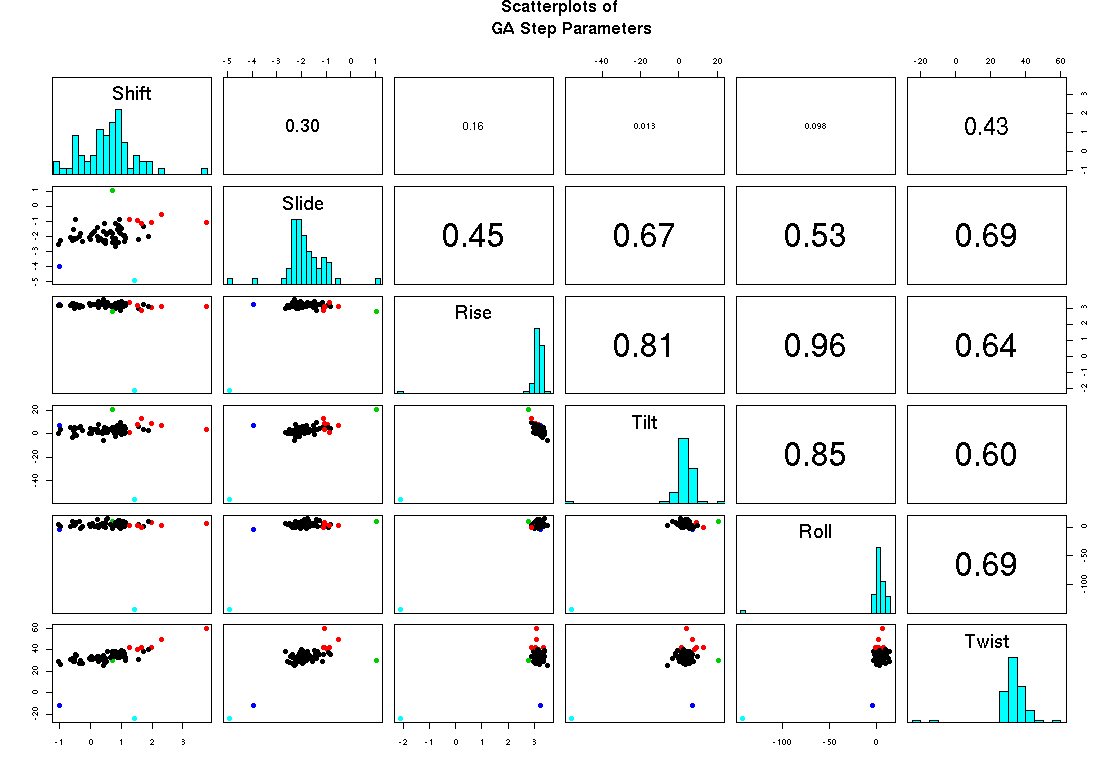
\includegraphics[angle=90, scale=0.6]{WC/GA.png}
\caption{Scatterplots for step-parameters of \textbf{WC} GA dinucleotide steps
in 50S rRNA.}
\label{fig:stepsGA}
\end{figure}

\begin{figure}[H]
\centering
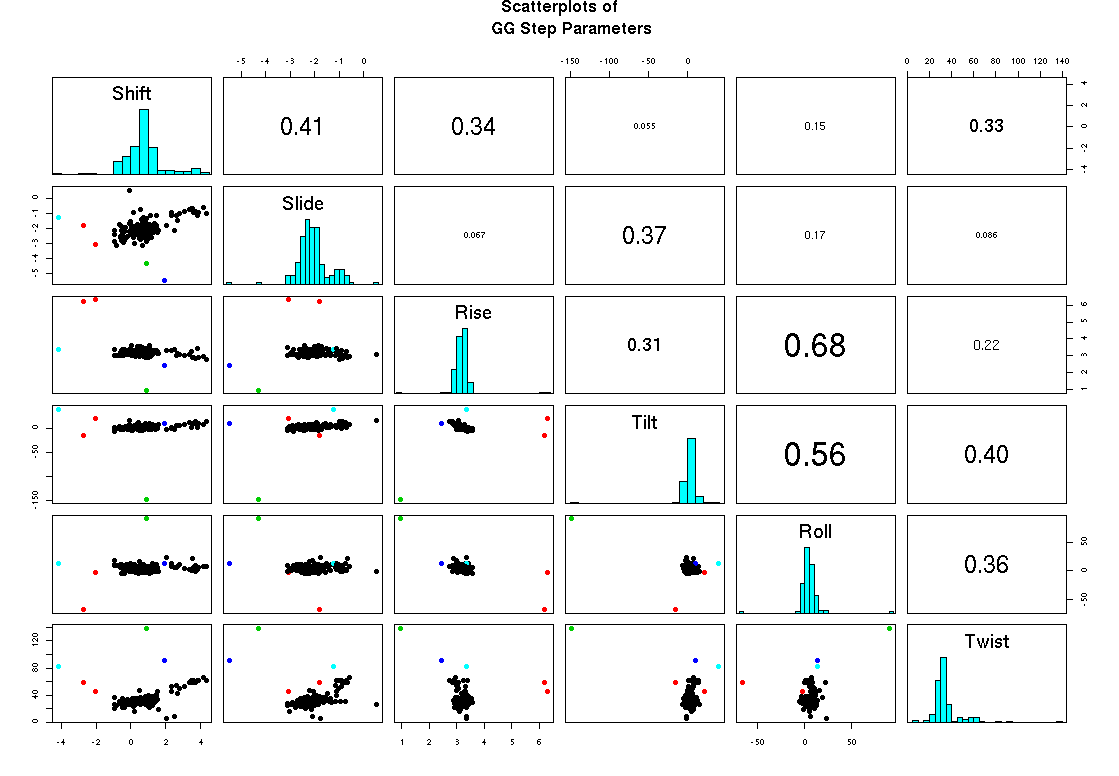
\includegraphics[angle=90, scale=0.6]{WC/GG.png}
\caption{Scatterplots for step-parameters of \textbf{WC} GG dinucleotide steps
in 50S rRNA.}
\label{fig:stepsGG}
\end{figure}

\begin{figure}[H]
\centering
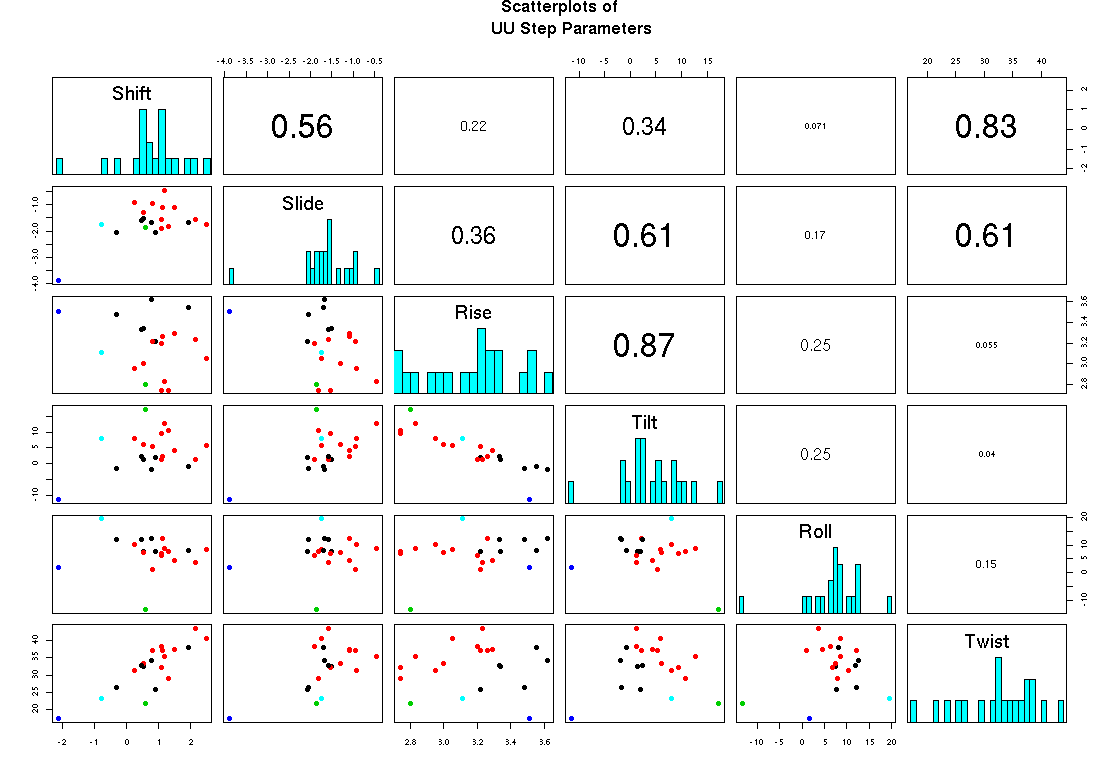
\includegraphics[angle=90, scale=0.6]{WC/UU.png}
\caption{Scatterplots for step-parameters of \textbf{WC} UU dinucleotide steps
in 50S rRNA.}
\label{fig:stepsUU}
\end{figure}

\begin{figure}[H]
\centering
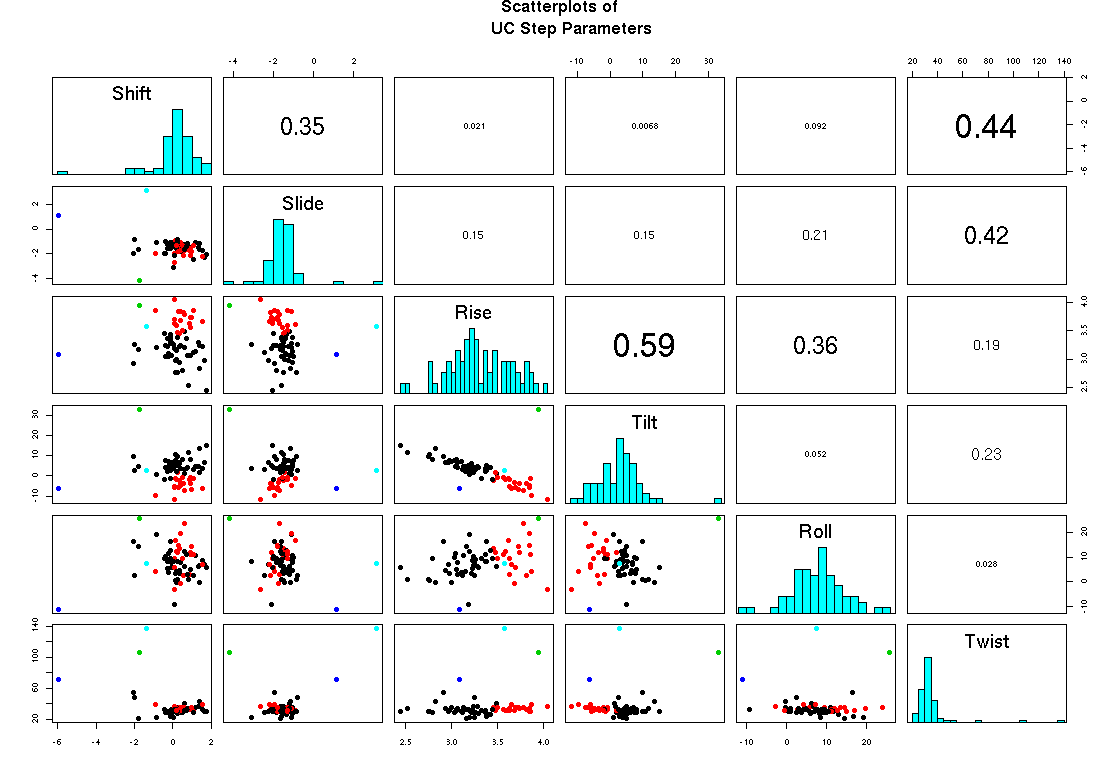
\includegraphics[angle=90, scale=0.6]{WC/UC.png}
\caption{Scatterplots for step-parameters of \textbf{WC} UC dinucleotide steps
in 50S rRNA.}
\label{fig:stepsUC}
\end{figure}

\begin{figure}[H]
\centering
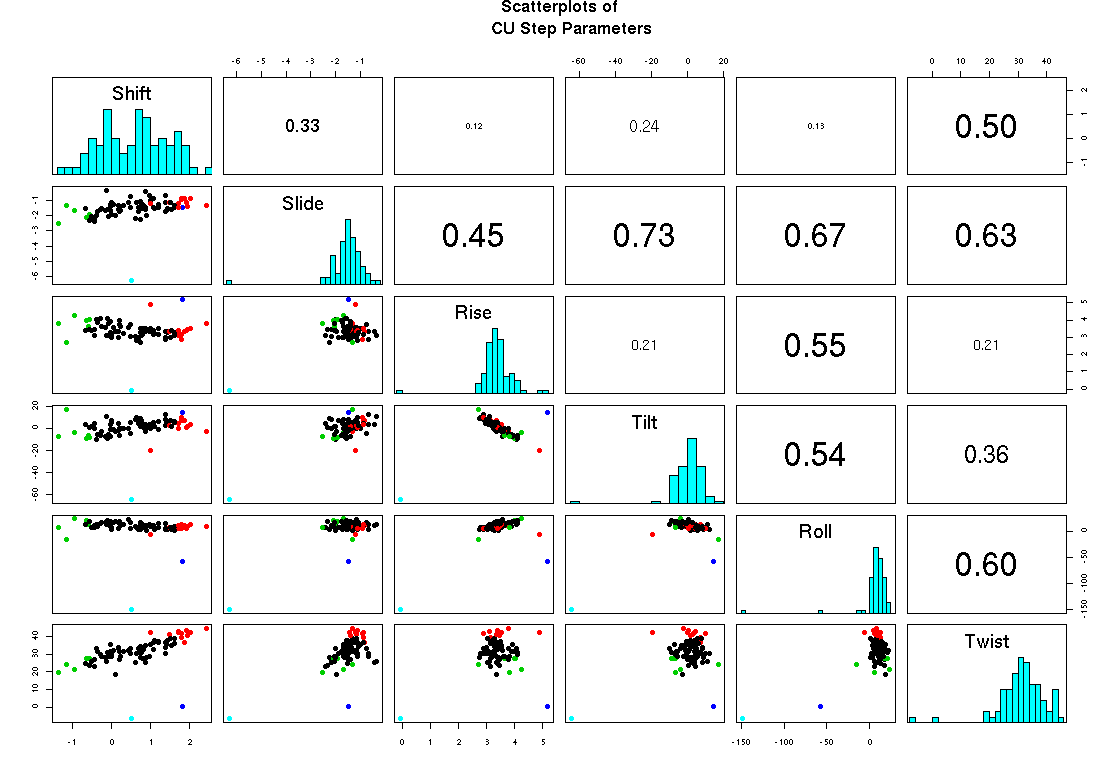
\includegraphics[angle=90, scale=0.6]{WC/CU.png}
\caption{Scatterplots for step-parameters of \textbf{WC} CU dinucleotide steps
in 50S rRNA.}
\label{fig:stepsCU}
\end{figure}

\begin{figure}[H]
\centering
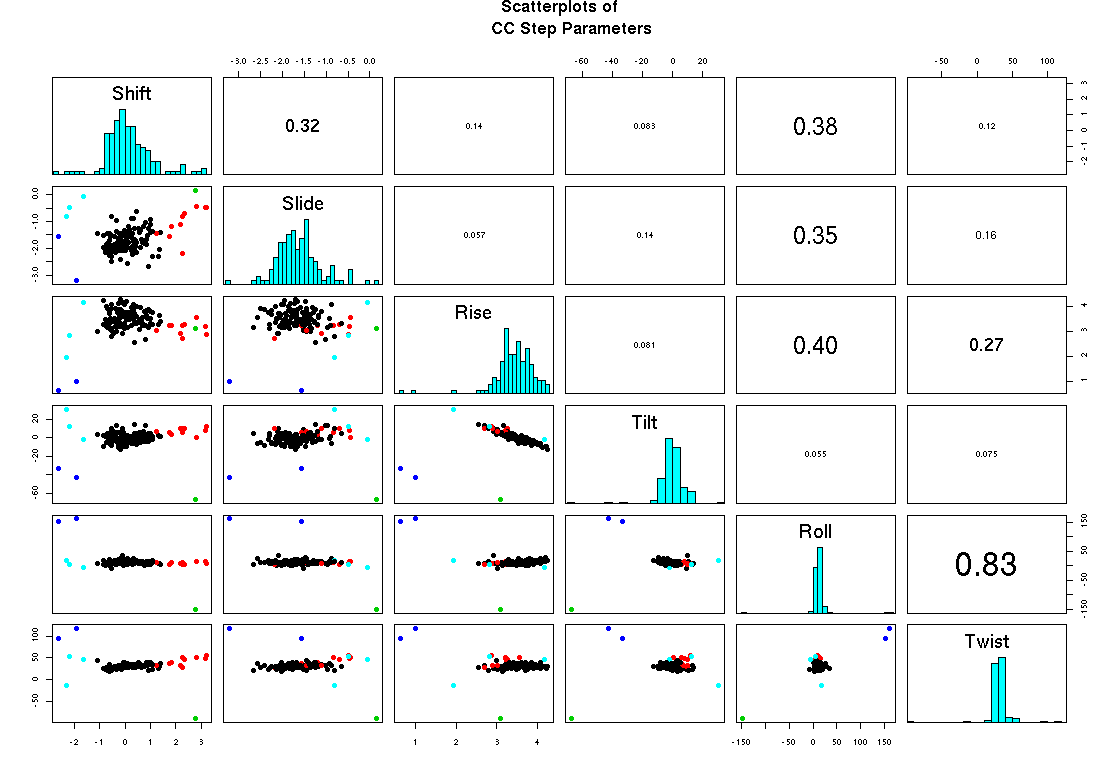
\includegraphics[angle=90, scale=0.6]{WC/CC.png}
\caption{Scatterplots for step-parameters of \textbf{WC} CC dinucleotide steps
in 50S rRNA.}
\label{fig:stepsCC}
\end{figure}

\begin{figure}[H]
\centering
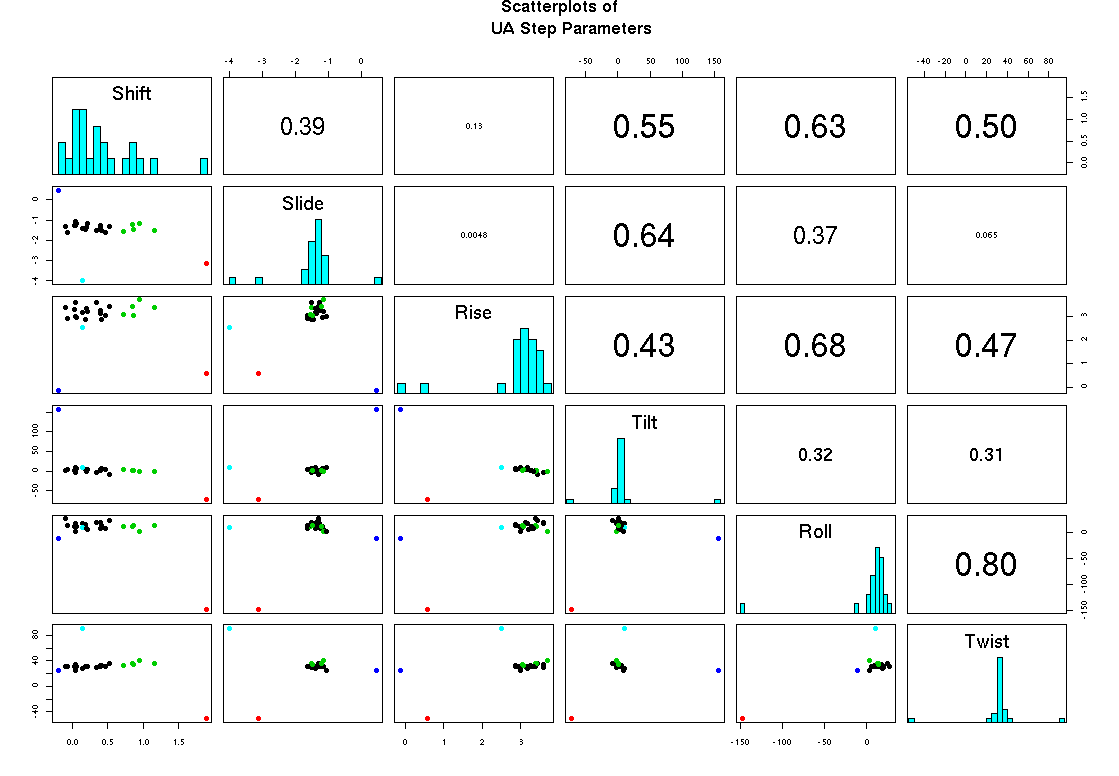
\includegraphics[angle=90, scale=0.6]{WC/UA.png}
\caption{Scatterplots for step-parameters of \textbf{WC} UA dinucleotide steps
in 50S rRNA.}
\label{fig:stepsUA}
\end{figure}

\begin{figure}[H]
\centering
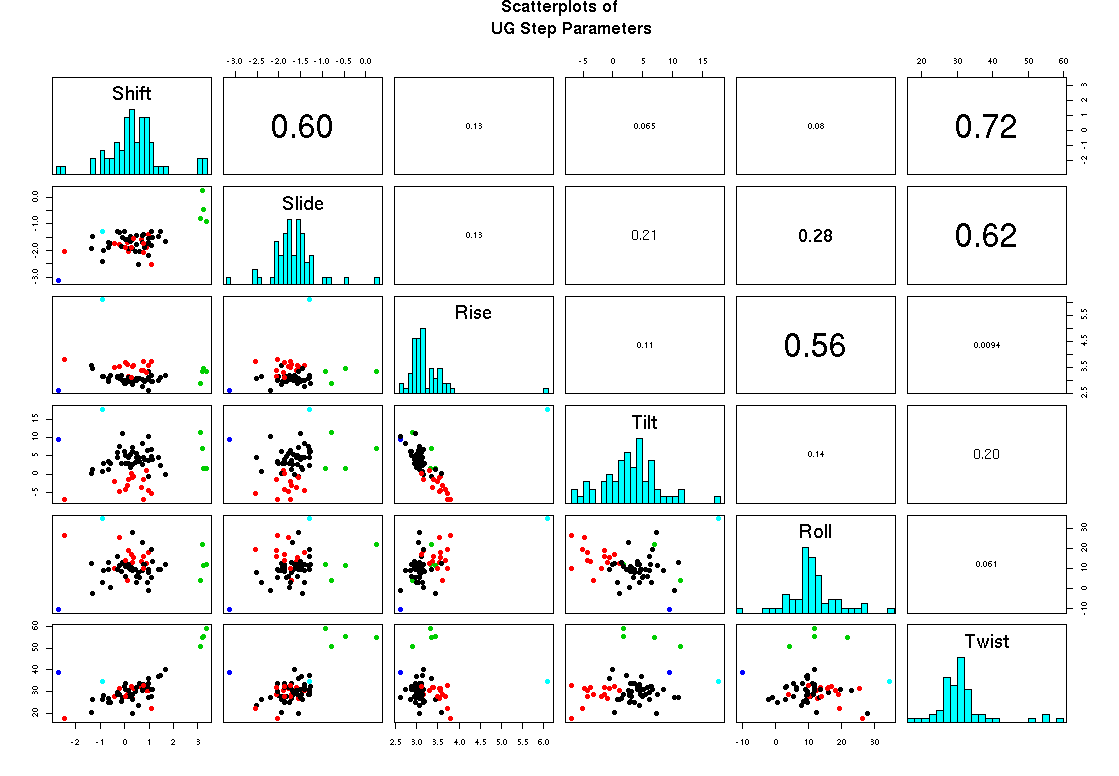
\includegraphics[angle=90, scale=0.6]{WC/UG.png}
\caption{Scatterplots for step-parameters of \textbf{WC} UG dinucleotide steps
in 50S rRNA.}
\label{fig:stepsUG}
\end{figure}

\begin{figure}[H]
\centering
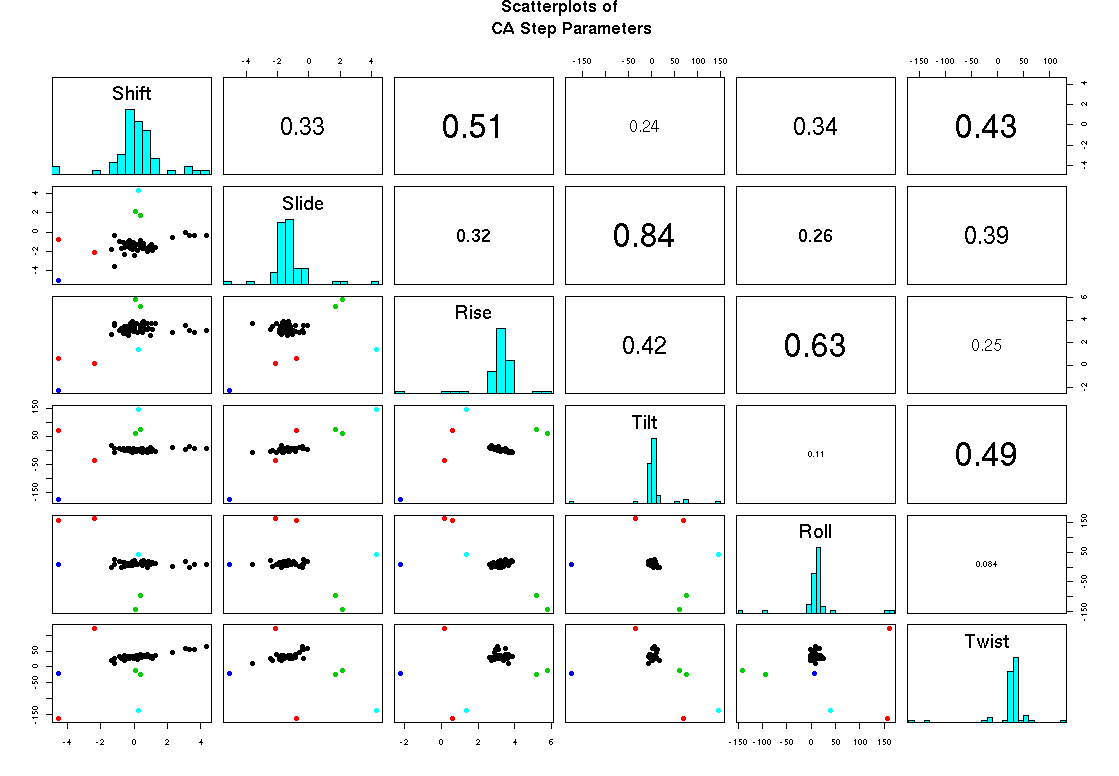
\includegraphics[angle=90, scale=0.6]{WC/CA.png}
\caption{Scatterplots for step-parameters of \textbf{WC} CA dinucleotide steps
in 50S rRNA.}
\label{fig:stepsCA}
\end{figure}

\begin{figure}[H]
\centering
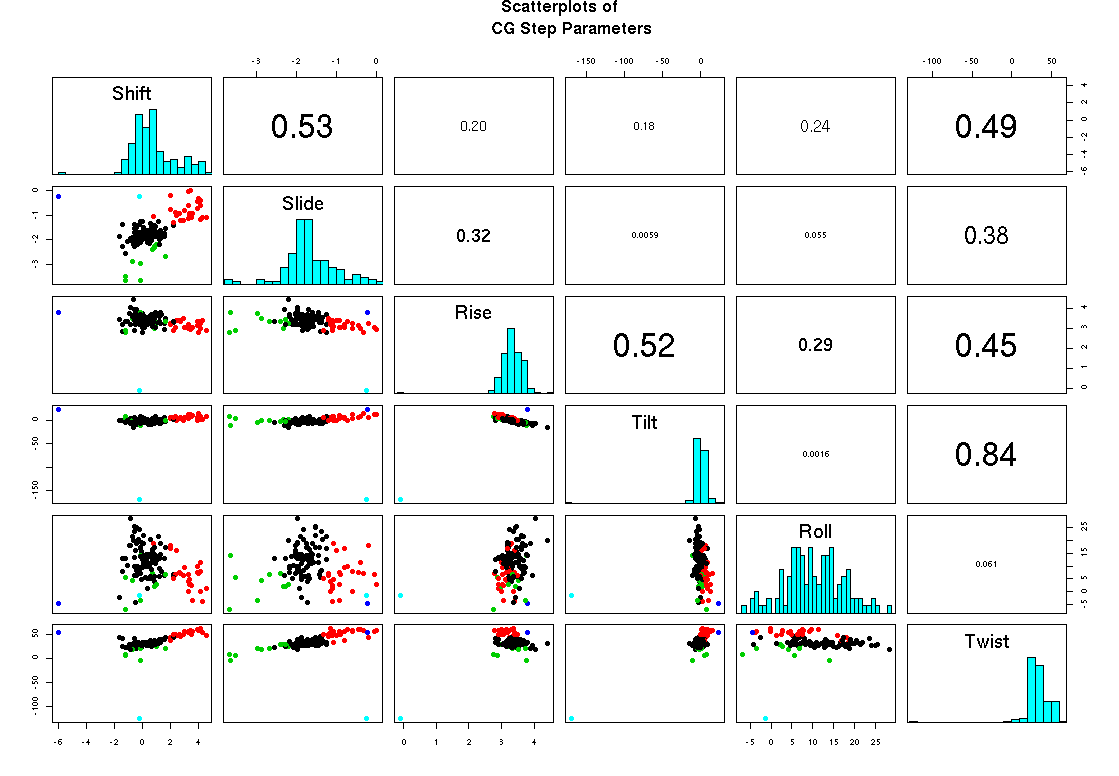
\includegraphics[angle=90, scale=0.6]{WC/CG.png}
\caption{Scatterplots for step-parameters of \textbf{WC} CG dinucleotide steps
in 50S rRNA.}
\label{fig:stepsCG}
\end{figure}

\begin{figure}[H]
\centering
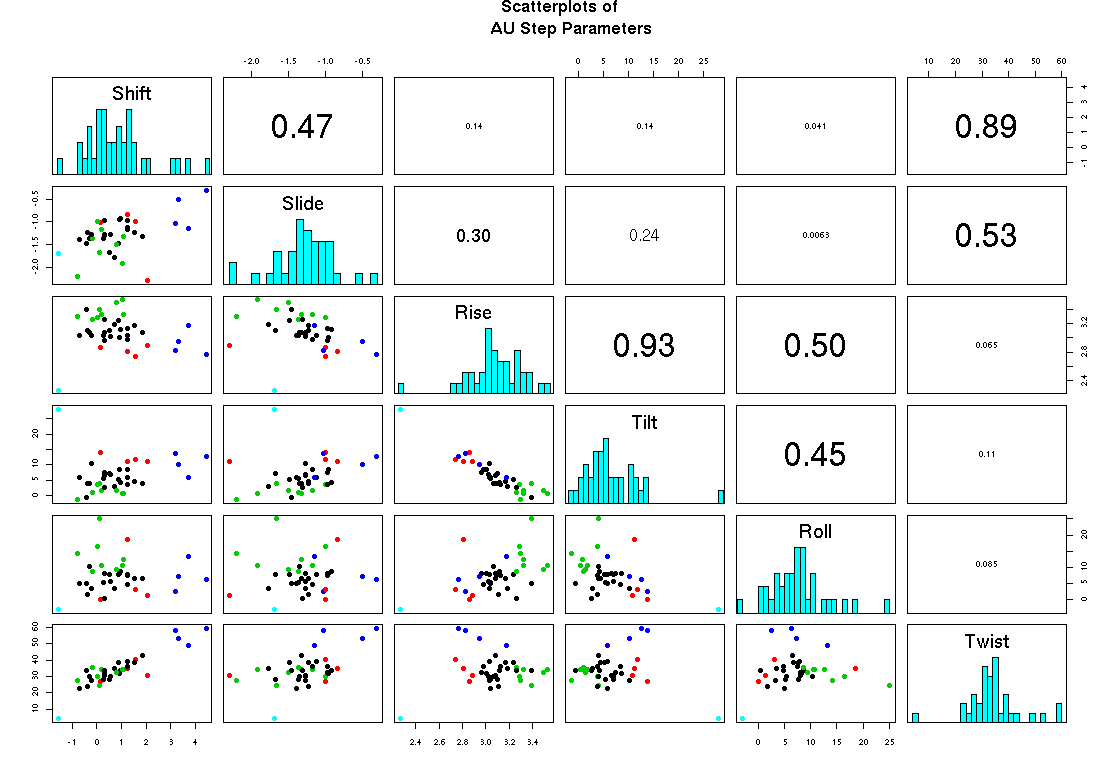
\includegraphics[angle=90, scale=0.6]{WC/AU.png}
\caption{Scatterplots for step-parameters of \textbf{WC} AU dinucleotide steps
in 50S rRNA.}
\label{fig:stepsAU}
\end{figure}

\begin{figure}[H]
\centering
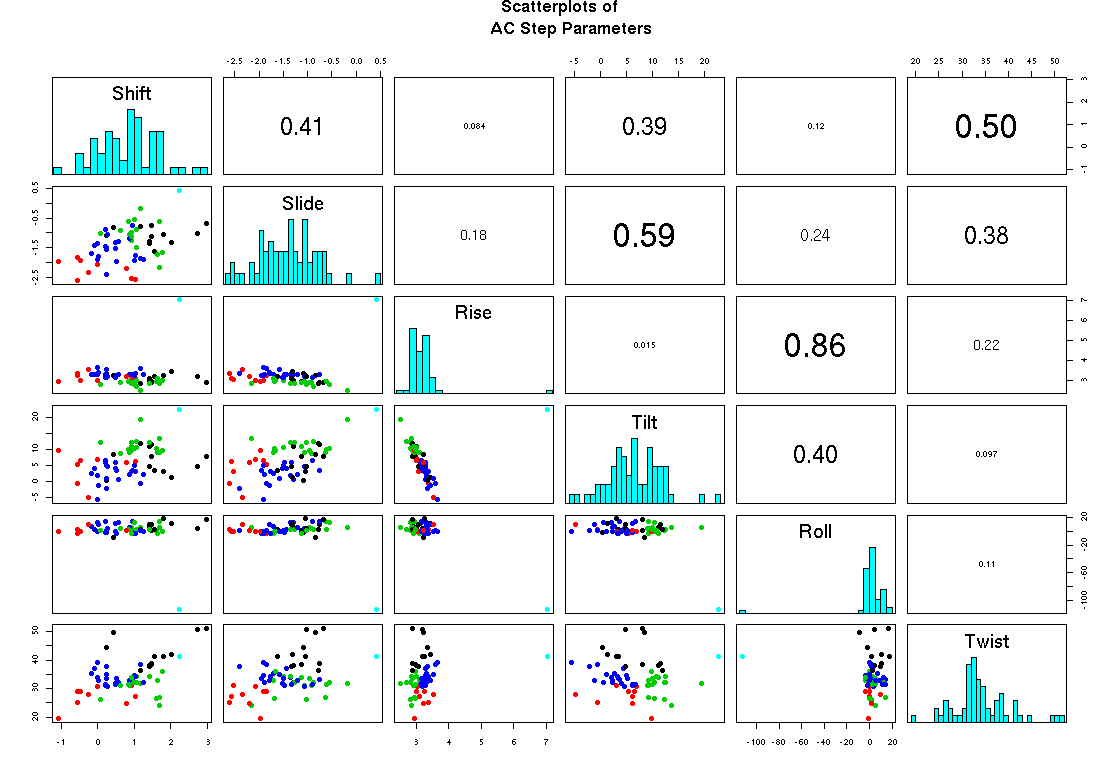
\includegraphics[angle=90, scale=0.6]{WC/AC.png}
\caption{Scatterplots for step-parameters of \textbf{WC} AC dinucleotide steps
in 50S rRNA.}
\label{fig:stepsAC}
\end{figure}

\begin{figure}[H]
\centering
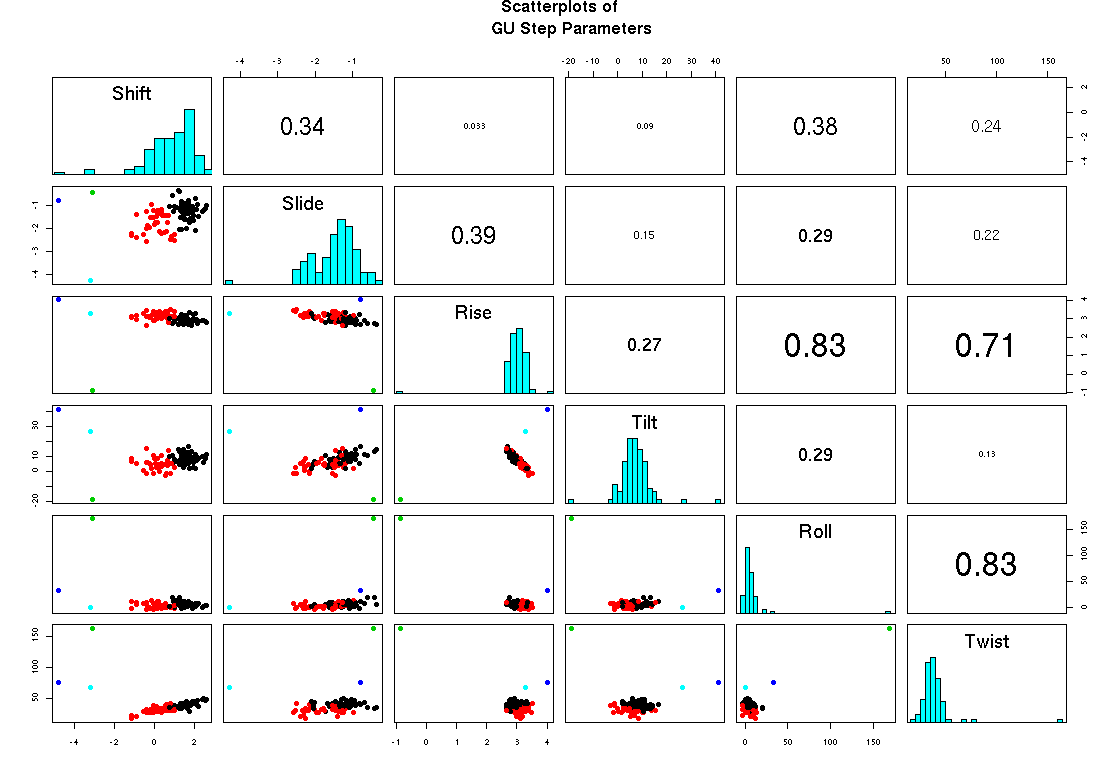
\includegraphics[angle=90, scale=0.6]{WC/GU.png}
\caption{Scatterplots for step-parameters of \textbf{WC} GU dinucleotide steps
in 50S rRNA.}
\label{fig:stepsGU}
\end{figure}

\begin{figure}[H]
\centering
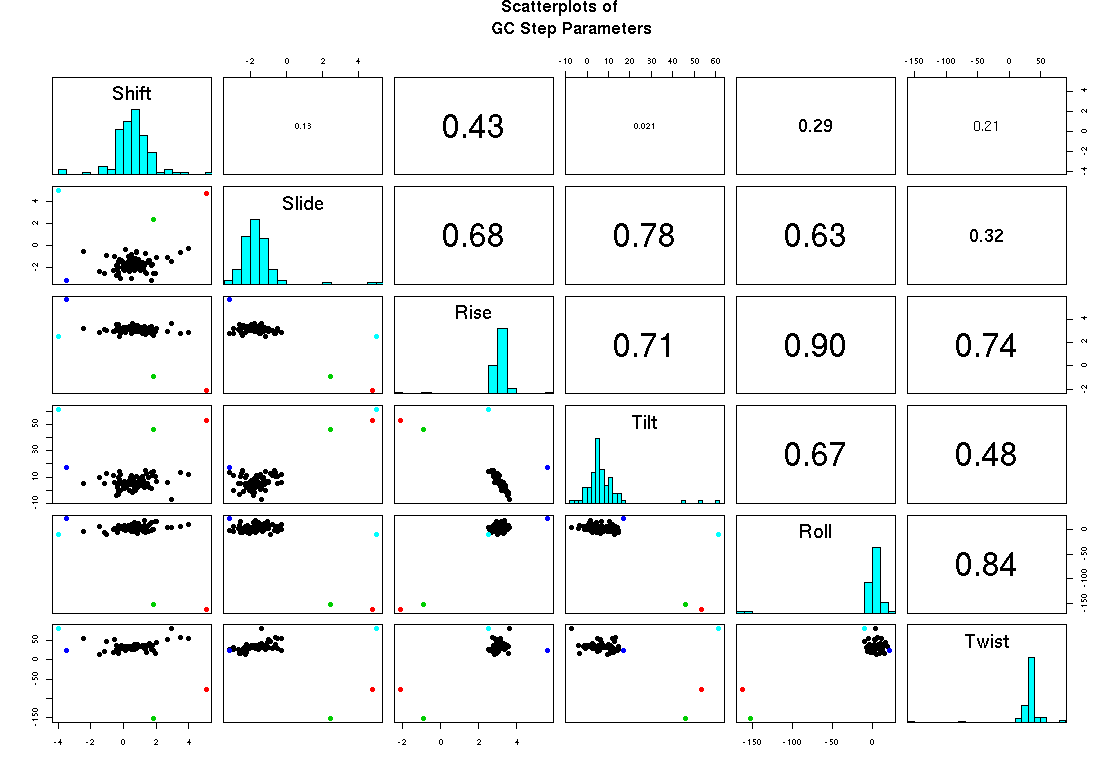
\includegraphics[angle=90, scale=0.6]{WC/GC.png}
\caption{Scatterplots for step-parameters of \textbf{WC} GC dinucleotide steps
in 50S rRNA.}
\label{fig:stepsGC}
\end{figure}

%\section{}

%\bibliography{biblio}
\printindex
